\article{$p$ 进群的表示：综述}{Representations of $p$-adic groups: A survey}{P. Cartier}{1}{111--155}
\section*{引言（Introduction）}
本文综述局部域（local field）上约化代数群（reductive algebraic group）表示论的部分已有成果，重点是无限维表示。研究对象包括常见的 $p$ 进群（$p$-adic group），如 $\GL_n(\Q_p),\operatorname{Sp}_{2n}(\Q_p),\ldots$。

这一理论起步较晚，发展缓慢。约在1960年，Mautner 及其学生率先展开研究，详细考察了具体例子 $\GL_2(\Q_p)$。最初的一般结果由 Bruhat [8] 及 Satake 得到：前者沿用了自己在学位论文 [7] 中处理实群的方法，后者确定了球面函数（spherical function）[38]。此后的进一步发展，则有赖于 Bruhat 与 Tits [10]、[11]、[12]、[13] 关于 $p$ 进约化群结构的深刻结果。

Jacquet 与 Langlands 在主要讨论 $\GL_2$ 的经典著作 [34] 中，引入了容许表示（admissible representation）这一重要概念，从而为这些表示的纯代数理论开辟道路。不久以后，Jacquet [32] 得到了关于诱导表示（induced representation）的基本结果。他只考虑 $\GL_n$，但所用方法完全一般。这些结果已由 Casselman 与 Harish-Chandra 推广。

本文的主要目标是描述和研究主系列（principal series）与球面函数。以下两个方向仍是当时研究的重点，但本文仅略作涉及：
\begin{enumerate}
\item[(a)] $p$ 进 Lie 群上的 Plancherel 定理及详细的调和分析（harmonic analysis）。Harish-Chandra 在这一领域起了主导作用。读者可参阅 Harish-Chandra 对自己结果的介绍 [26]、[27]；关于 Harish-Chandra 和 Roger Howe 更近期的结果，也可参阅我的 Bourbaki 讲座 [14]。
\item[(b)] 绝对尖点表示（absolutely cuspidal representation，即所谓“离散系列”，discrete series）的显式构造。\footnote{\textbf{译者注（本次校订）：}本文在这里及2.4将“离散系列”用于绝对尖点表示。按通常的表示论术语，绝对尖点（超尖点）表示与模中心平方可积的离散系列并不相同：酉超尖点表示属于离散系列，反向包含一般不成立。例如 $\GL_2(F)$ 的 Steinberg 表示模中心平方可积，但并非超尖点。2.5另行定义了平方可积表示。}Shintani [40]、Gérardin [21] 和 Howe（即将在 Pacific J. Math. 发表的文章）在此取得了重要进展。这一方向已初步显现出一些深刻的算术问题，可以预见它们的研究将相当困难。
\end{enumerate}
本文的内容安排如下。第 I 节在一般框架下介绍各类表示。遵循 Harish-Chandra [25]，针对全不连通局部紧群（totally disconnected locally compact group）给出定义。数论与自守函数提供大量这样的群及其表示。特别关注各种形式的 Frobenius 互反律（Frobenius reciprocity）及各种诱导表示概念。叙述采用一种似乎尚未使用过的张量积方法；这一方法需要在无单位元的环上取张量积。

第 II 节建立一套工具，依照 Jacquet，将 $p$ 进群 $G$ 的不可约容许表示分类化约为以下两个问题：
\begin{enumerate}
\item[(a)] 构造 $G$ 及其抛物子群（parabolic subgroup）的 Levi 分量的绝对尖点不可约表示；
\item[(b)] 研究从抛物子群到整个群的诱导表示。
\end{enumerate}
我们将利用前面对诱导表示的描述，介绍 Jacquet 的两个基本构造，即“Jacquet 函子”（Jacquet functor）。这种表述比通常的处理更为对称。将先前结果专门用于 $\GL_n$ 的经典情形后，转向酉表示（unitary representation）和容许表示之间的关系。基本结果归功于 Harish-Chandra [28]（推广了 R. Howe 关于 $\GL_n$ 的较早结果 [29]）和 Bernshtein [1]。它们说明，局部域上的任意约化代数群，在 von Neumann--Murray 分类的意义下都属于 I 型（type I），这为建立 Plancherel 定理奠定了基础。

第 III 节讨论非分歧主系列（unramified principal series）。这些表示由极小抛物子群的 Levi 分量的所谓非分歧特征（unramified character）参数化。这些特征在将表示论应用于 Langlands 的 $L$ 群（$L$-group）理论时起着关键作用（见本论文集中 Borel 的讲座）。通常这一系列中的表示 $I(\chi)$ 不可约。它们总有在某个特殊极大紧子群下不变的非零向量。主要结果是显式构造 $I(\chi)$ 与 $I(w\chi)$ 之间的等价映射，其中 $w$ 为（相对）Weyl 群的元素。在实 Lie 群情形，这一问题导致了奇异积分算子（singular integral operator）的引入（Stein、Knapp）。Casselman 的一个极为巧妙的技巧充分利用 Jacquet 构造 $V\mapsto V_N$，绕过了构造这些算子所涉及的深刻分析问题。Iwahori 子群（Iwahori subgroup）及其在建筑（building）中的几何解释，也将在这一过程中发挥重要作用。

第 IV 节讨论球面函数理论，汇集前面各节的结果。利用第 III 节阐述的结果，可重新得到这些球面函数的 Macdonald 公式 [36]、[37]。这一理论在实 Lie 群情形已高度发展。从表示论的角度看，球面主系列是一类较特殊的表示；在 Langlands 理论的 $L$ 函数研究中，它们却十分重要。

第 III、IV 节研究球面函数所用的整套方法，来自 Casselman 尚未发表的文章 [18]。我大量借鉴了该文及同一作者建立 $p$ 进情形表示论基础的初步论文 [17]。读者需参阅这些文章了解证明细节与众多推广。希望它们不久能够发表。

我要感谢几位朋友。Anna Helversen-Pasotto 将我的讲座录音，并根据录音整理口述文字。这项繁琐的整理工作，为我将会议期间分发的简略讲义扩写成本文提供了很大帮助。

Serge Lang 与 John Tate 允许我自由使用他们关于球面变换的笔记，第 IV 节的处理受到了他们的影响。John Tate 还纠正了我对 Frobenius 互反律的误解（见1.7）。
\section*{记号与约定（Notations and conventions）}
\paragraph*{1.}
设 $A$ 为带单位元 $1$ 的环。令 $A^\times$ 为 $A$ 中满足存在 $b\in A$ 使 $ab=1$ 的元素 $a$ 的集合。以环中的乘法为运算，$A^\times$ 构成群，称为 $A$ 的“乘法群”（multiplicative group）。\footnote{\textbf{译者注（本次校订）：}一般非交换环中，定义可逆元必须要求 $ab=ba=1$；仅有右逆 $ab=1$ 不够。例如在以 $e_0,e_1,\ldots$ 为基的向量空间上，令 $S(e_i)=e_{i+1}$，$T(e_0)=0$、$T(e_{i+1})=e_i$，则 $TS=1$ 而 $ST\ne1$。因此本段定义中的条件应补为双边逆元条件。}
\paragraph*{2.}
设 $M$ 为无单位元环 $A$ 上的模。若 $M$ 中每个元素均可写成 $a_1m_1+\cdots+a_km_k$，其中 $a_1,\ldots,a_k\in A$，$m_1,\ldots,m_k\in M$，则称 $M$ 非退化（nondegenerate）。\footnote{约定带单位元环上的任意含幺模都是非退化的。}

若 $M$ 中任意元素都能表示为 $a_1m_1+\cdots+a_km_k+n_1m_1+\cdots+n_km_k$，其中 $a_i\in A$，$n_i$ 为任意正负整数，就说元素列 $m_1,\ldots,m_k$ 生成 $M$。若 $M$ 非退化，可省略各项 $n_1m_1,\ldots,n_km_k$。若存在生成 $M$ 的有限列，则称模 $M$ 有限生成（finitely generated）。
\paragraph*{3.}
本文所谓局部域，指剩余域（residue field）有限的非阿基米德局部域。这样的域 $F$ 配备一个子环 $\mathfrak O_F$，其元素称为 $F$ 中的整数（integer）。$\mathfrak O_F$ 中存在唯一非零素理想 $\mathfrak p_F$，并且存在素元（prime element）$\widetilde\omega_F\in\mathfrak O_F$，使 $\mathfrak p_F=\mathfrak O_F\widetilde\omega_F$。每个 $x\in F^\times$ 都可唯一写成 $\widetilde\omega_F^n u$，其中 $n$ 为某个整数，$u\in\mathfrak O_F^\times=\mathfrak O_F\setminus\mathfrak p_F$。此时令 $\operatorname{ord}_F(x)=n$；约定 $\operatorname{ord}_F(0)=+\infty$。指数 $q=(\mathfrak O_F:\mathfrak p_F)$ 有限，且为某个素数 $p$ 的幂。对 $x\in F^\times$ 令 $|x|_F=q^{-\operatorname{ord}_F(x)}$，并令 $|0|_F=0$。不会混淆时，$\mathfrak O_F,\mathfrak p_F,\mathfrak O_F^\times,\widetilde\omega_F,\operatorname{ord}_F(x),|x|_F$ 中的下标 $F$ 可以省略。

有两种可能：
\begin{enumerate}
\item[(a)] 若 $F$ 特征为零，则 $F$ 为 $p$ 进域 $\Q_p$ 的有限代数扩张，$\mathfrak O_F$ 由在 $p$ 进整数环 $\Z_p$ 上整的元素组成。
\item[(b)] 若 $F$ 特征为 $p$，则 $F$ 为环 $\mathfrak O_F=\F_q[[t]]$ 的分式域（quotient field）；该环由一个不定元 $t$ 的形式幂级数（formal power series）组成，系数属于 Galois 域 $\F_q$（某些作者亦记为 $\operatorname{GF}(q)$）。
\end{enumerate}
\paragraph*{4.}
采用标准记号：$\Z$ 表示整数环，$\Q$ 表示有理数域，$\R$ 表示实数域，$\C$ 表示复数域。
\paragraph*{5.}
设 $G$ 为拓扑群，单位元记为 $1$。$G$ 的特征（character）指任意连续同态 $\chi:G\to\C^\times$。若对每个 $g\in G$，复数 $\chi(g)$ 的模为 $1$，即
\[
\overline{\chi(g)}=\chi(g)^{-1}=\chi(g^{-1}),
\]
则称 $\chi$ 为酉特征（unitary character）。\footnote{有些作者将本文所谓“特征”称为“拟特征”（quasi-character），而将本文所谓“酉特征”称为“特征”。}

假定 $G$ 局部紧。以 $C_c(G)$ 表示 $G$ 上连续紧支集复值函数空间。若 $\mu$ 为 $G$ 上的（左不变）Haar 测度，通常以 $\int_Gf(g)\,dg$ 表示 $f\in C_c(G)$ 关于 $\mu$ 的积分。模函数（modular function）$\Delta_G$ 由积分规则
\[
\int_G f(g)\,dg=\Delta_G(g_0)\int_G f(gg_0)\,dg,\qquad f\in C_c(G),
\]
刻画。若 $\Delta_G=1$，称群 $G$ 幺模（unimodular）。

有时需在齐性空间（homogeneous space）$G/H$ 上积分。设 $f$ 是 $G$ 上连续函数，且存在 $f_1\in C_c(G/H)$，使任意 $g\in G$ 满足 $f(g)=f_1(gH)$。选取 $G/H$ 上的不变测度 $\mu$。\footnote{\textbf{译者注（本次校订）：}这里需假定 $H$ 闭，且 $G/H$ 存在非零的 $G$ 不变 Radon 测度；其充要条件为 $\Delta_G|_H=\Delta_H$。例如后文的 $G/Z$ 满足此条件，因为 $Z$ 是中心子群。}$f_1$ 关于 $\mu$ 的积分常记为 $\int_{G/H}f(g)\,d\bar g$。

若 $G$ 为（实或 $p$ 进）Lie 群，以相应的德文字母 $\mathfrak g$ 表示其 Lie 代数。
\paragraph*{6.}
设 $X$ 为任意集合。$X$ 中的恒等映射记为 $1_X$。若 $A$ 是 $X$ 的任意子集，示性函数（characteristic function）$I_A:X\to\{0,1\}$ 定义为：$x\in A$ 时 $I_A(x)=1$，$x\in X\setminus A$ 时 $I_A(x)=0$；$X\setminus A$ 表示集合差。

若 $X$ 有限，其基数（cardinality）记为 $|X|$。
\paragraph*{7.}
使用缩写“iff”表示“当且仅当”（if and only if），“w.r.t.”表示“关于”（with respect to）。
\origsection{I}{全不连通群及其表示（Totally disconnected groups and their representations）}
\origsubsection{1.1}{td 型群（Groups of td-type）}
设 $G$ 为拓扑群。若其单位元 $1$ 的每个邻域都包含一个紧开子群，称 $G$ 为 td 型（td-type）。这样的群是局部紧 Hausdorff 空间，并且全不连通（totally disconnected，故简记 td），即 $G$ 中不存在含多于一个元素的连通子集。

设 $G$ 为 td 型群。若 $X_1,X_2$ 为 $G$ 中非空紧开集，则存在 $G$ 的紧开子群 $K$，使 $X_1,X_2$ 都是有限多个陪集之并：分别为 $x_{1,1}K,\ldots,x_{1,n_1}K$ 与 $x_{2,1}K,\ldots,x_{2,n_2}K$。令
\[
(X_1:X_2)=n_1/n_2.\tag{1}
\]
例如，若 $X_1,X_2$ 为紧开子群且 $X_2\subseteq X_1$，则 $(X_1:X_2)$ 为 $X_2$ 在 $X_1$ 中的指数。链式法则成立，即
\[
(X_1:X_3)=(X_1:X_2)(X_2:X_3).\tag{2}
\]
设 $\mu$ 为 $G$ 上左不变 Haar 测度。显然有
\[
(X_1:X_2)=\mu(X_1)/\mu(X_2).\tag{3}
\]
因此，若对某个紧开非空集 $X$，$\mu(X)$ 为有理数，则对每个这样的集合均然。满足这一条件的 Haar 测度 $\mu$ 称为有理测度（rational）。
\origsubsection{1.2}{td 型群的例子（Examples of groups of td-type）}
（a）设 $G$ 为 td 型群，则 $G$ 的每个开子群、每个闭子群都是 td 型，$G$ 对闭正规子群的商群也是 td 型。

（b）若 $G_1,\ldots,G_n$ 是 td 型群，其赋予积拓扑的直积 $G_1\times\cdots\times G_n$ 也是 td 型。

（c）设 $(G_i)_{i\in I}$ 为 td 型群的任意无限族，并对每个 $i\in I$ 选取紧开子群 $K_i\subseteq G_i$。在直积 $\prod_{i\in I}G_i$ 中，令 $G$ 为由满足 $\{i\in I\mid g_i\notin K_i\}$ 有限的族 $(g_i)_{i\in I}$ 组成的子群。于是 $K=\prod_{i\in I}K_i$ 是 $G$ 的子群。先在 $K$ 上取积拓扑。$G$ 中集合 $U$ 为开集，当且仅当对每个 $g\in G$，$gU\cap K$ 在 $K$ 中开。此时 $G$ 是 td 型群，$K$ 为其紧开子群。群 $G$ 称为各群 $G_i$ 关于各群 $K_i$ 的限制直积（restricted product）。

（d）设 $F$ 为局部域。$|x-y|_F$ 在 $F$ 中定义距离，从而定义拓扑。则 $F$ 的加法群为 td 型，$\mathfrak O_F$ 为紧开子群。而且 $F^\times$ 在 $F$ 中开，因此其乘法群为 td 型，$\mathfrak O_F^\times$ 为紧开子群。

（e）设整数 $n\geq1$。线性群 $\GL_n(F)$ 为以 $x_{11},x_{12},\ldots,x_{nn}$ 为坐标的 $n^2$ 维 $F$ 空间中，由 $\det(x_{ij})\ne0$ 定义的开子空间。它是 td 型群。一个紧开子群为 $\GL_n(\mathfrak O_F)$，即元素属于 $\mathfrak O_F$、行列式属于 $\mathfrak O_F^\times$ 的 $n$ 阶矩阵集合。

（f）设 $G$ 为 $\GL_n(F)$ 的子群，由坐标 $x_{ij}$ 的一组 $F$ 系数多项式的公共零点定义。简称 $G$ 是 $\GL_n(F)$ 的代数子群（algebraic subgroup），更精确地，是某个定义在 $F$ 上的代数群的 $F$ 有理点集合。它是 $\GL_n(F)$ 的闭子群，故本身是 td 型群。$G$ 中单位矩阵 $I_n$ 的邻域基由子群
\[
K_m=\{g=(g_{ij})\in G\mid|g_{ij}-\delta_{ij}|_F\leq q^{-m}\ (1\leq i,j\leq n)\}
\]
给出。

设 $G'$ 为某个 $\GL_{n'}(F)$（$n'\geq1$）的代数子群。假定群同态 $\rho:G\to G'$ 有理，即存在 $\rho_{kl}\in F[X_{11},\ldots,X_{nn}]$ 和整数 $m\geq1$，使对 $g=(g_{ij})\in G$ 有
\[
\rho(g)=\left(\frac{\rho_{kl}(g_{11},\ldots,g_{nn})}{(\det g)^m}\right)_{1\leq k,l\leq n'}.
\]
则 $\rho$ 关于 $G,G'$ 分别嵌入 $\GL_n(F),\GL_{n'}(F)$ 所定义的拓扑连续。特别地，若 $\rho$ 为双正则同构（biregular isomorphism），即 $\rho$ 是群同构且 $\rho,\rho^{-1}$ 均有理，则 $\rho$ 为同胚。

更内在地说，$G$ 上的代数结构由多项式函数环 $F[G]$ 定义，\footnote{此环由函数 $g\mapsto u(g_{11},\ldots,g_{nn})/(\det g)^m$ 组成，其中 $u\in F[X_{11},\ldots,X_{nn}]$，整数 $m\geq0$。}而上述拓扑是使 $F[G]$ 的元素都成为 $G$ 到 $F$ 的连续映射的最粗拓扑（$F$ 带有（d）定义的拓扑）。

（g）由（b）、（f），在相同或不同局部域上定义的有限多个代数群之积为 td 型。同样由（c）、（f），不含阿基米德分量的阿代尔群为 td 型。
（h）设 $F$ 为局部域，$F_{\mathrm{sep}}$ 为 $F$ 的可分代数闭包（separable algebraic closure），$F_{\mathrm{unr}}$ 为包含于 $F_{\mathrm{sep}}$ 的 $F$ 的极大非分歧扩张，$\sigma$ 为 $F_{\mathrm{unr}}/F$ 的 Frobenius 自同构。令 $G_F=\Gal(F_{\mathrm{sep}}/F)$ 为赋予 Krull 拓扑的 Galois 群。它是紧 td 型群。令 $W_F\subseteq G_F$ 为由在 $F_{\mathrm{unr}}$ 上诱导某个 $\sigma^n$ 的 $F_{\mathrm{sep}}$ 自同构 $\varphi$ 组成的子群。$F$ 的 Weil 群（Weil group）$W_F$ 上存在唯一的 td 型群拓扑，使 $\Gal(F_{\mathrm{sep}}/F_{\mathrm{unr}})$（带 Krull 拓扑）为 $W_F$ 的紧开子群。
\origsubsection{1.3}{Hecke 代数（Hecke algebra）}
设 $G$ 为 td 型群。对 $G$ 的任意紧开子群 $K$，以 $\mathcal H(G,K)$ 表示 $G$ 上满足下述两个条件的复值函数 $f$ 构成的复向量空间：
\begin{enumerate}
\item[(a)] $f$ 在 $K$ 下双不变，即 $f(kgk')=f(g)$（$g\in G,k,k'\in K$）；
\item[(b)] $f$ 在有限多个双陪集 $KgK$ 的并之外为零。
\end{enumerate}
再选取 $G$ 上（左不变）Haar 测度 $\mu$。用通常卷积公式在 $\mathcal H(G,K)$ 中定义双线性乘法：
\[
(f_1*f_2)(g)=\int_G f_1(x)f_2(x^{-1}g)\,dx.\tag{4}
\]
该积分有意义，因为作为 $x$ 的函数，被积函数局部常值且有紧支集。在这一乘法下，$\mathcal H(G,K)$ 成为复数域 $\C$ 上的结合代数。

选取 $G$ 模 $K$ 的双陪集代表集 $\{g_\alpha\}$，即 $G$ 为集合 $Kg_\alpha K$ 的不交并。对每个指标 $\alpha$，定义
\[
u_\alpha(g)=\begin{cases}\mu(K)^{-1},&g\in Kg_\alpha K,\\0,&\text{其他情形}.\end{cases}\tag{5}
\]
特别可假定某个指标 $0$ 对应 $g_0=1$，相应函数 $u_0$ 记为 $e_K$。因此
\[
e_K(g)=\begin{cases}\mu(K)^{-1},&g\in K,\\0,&\text{其他情形}.\end{cases}\tag{6}
\]
族 $\{u_\alpha\}$ 为向量空间 $\mathcal H(G,K)$ 的一组基。$e_K$ 为此代数的单位元，乘法表为 $u_\alpha*u_\beta=\sum_\gamma c_{\alpha\beta\gamma}u_\gamma$，其中系数按如下方式计算。群 $K_\alpha=K\cap g_\alpha Kg_\alpha^{-1}$ 紧开，因而在 $K$ 中指数有限。因此存在 $K$ 的元素 $x_1,\ldots,x_m$，使 $K$ 为各集合 $x_1K_\alpha,\ldots,x_mK_\alpha$ 的不交并；$Kg_\alpha K$ 因而为 $x_1g_\alpha K,\ldots,x_mg_\alpha K$ 的不交并。类似定义 $K_\beta$ 和元素 $y_1,\ldots,y_{m'}$。那么 $c_{\alpha\beta\gamma}$ 为使 $g_\gamma^{-1}x_i g_\alpha y_jg_\beta\in K$ 的有序对 $(i,j)$ 的数目（见 Shimura [39]）。

当 $K'$ 为 $K$ 的紧开子群时，$\mathcal H(G,K)$ 是 $\mathcal H(G,K')$ 的子环，但若 $K\ne K'$，两者的单位元不同。定义 $\mathcal H(G)=\bigcup_K\mathcal H(G,K)$，其中 $K$ 遍历由紧开子群组成的 $1$ 的一个邻域基。则 $\mathcal H(G)$ 就是 $G$ 上局部常值紧支集函数的空间。对 (4) 定义的卷积，$\mathcal H(G)$ 是结合代数；除非 $G$ 离散，它没有单位元；它交换当且仅当 $G$ 交换。

代数 $\mathcal H(G)$ 称为 $G$ 的 Hecke 代数，$\mathcal H(G,K)$ 称为 $G$ 关于 $K$ 的 Hecke 代数。\footnote{当 $G=\GL_2(\Q_p)$，$K=\GL_2(\Z_p)$ 时，这个代数就是与 $p$ 相联系的经典 Hecke 算子代数。}

为后文需要，推广 $\mathcal H(G)$。设 $Z$ 为 $G$ 的中心的闭子群，$\chi$ 为 $Z$ 的特征。以 $\mathcal H_\chi(G)$ 表示满足下列条件的复值函数集合：
\begin{enumerate}
\item[(a)] $f$ 局部常值；
\item[(b)] 对 $z\in Z,g\in G$，$f(zg)=\chi(z)^{-1}f(g)$；
\item[(c)] $f$ 模 $Z$ 后有紧支集。
\end{enumerate}
具体而言，条件 (c) 是说 $f$ 在形如 $\Omega Z$ 的集合之外为零，其中 $\Omega$ 在 $G$ 中紧。选取 $G/Z$ 上 Haar 测度 $\nu$。$\mathcal H_\chi(G)$ 中卷积乘法定义为
\[
(f_1*_\chi f_2)(g)=\int_{G/Z}f_1(x)f_2(x^{-1}g)\,d\bar x.\tag{7}
\]
注意当 $z\in Z$ 时，被积函数在 $x,xz$ 取值相同。这一乘法满足双线性和结合律。除非 $Z$ 在 $G$ 中开，代数 $\mathcal H_\chi(G)$ 没有单位元。当 $Z=\{1\}$，此构造回到 $\mathcal H(G)$。
\origsubsection{1.4}{光滑表示（Smooth representations）}
按通常约定，$G$ 的表示（representation）是一对 $(\pi,V)$，其中 $V$ 是复向量空间，$\pi$ 为从 $G$ 到 $V$ 中可逆线性映射群的同态。若 $H$ 为 $G$ 的子群，以 $V^H$ 表示满足对所有 $h\in H$ 有 $\pi(h)v=v$ 的向量 $v\in V$ 的空间，即在 $G$ 中稳定子包含 $H$ 的向量。
\begin{originaltheorem}{定义 1.1（Definition 1.1）}
$G$ 的表示 $(\pi,V)$ 称为光滑，若 $V$ 中每个向量的稳定子为开集；等价地，$V=\bigcup_K V^K$，其中 $K$ 遍历 $G$ 的紧开子群。
\end{originaltheorem}
设 $(\pi,V)$ 为 $G$ 的光滑表示，$V^*$ 为 $V$ 上所有线性形式的空间。$\pi$ 的系数（coefficient）$\pi_{v,v^*}$（$v\in V,v^*\in V^*$）定义为
\[
\pi_{v,v^*}(g)=\langle v^*,\pi(g)v\rangle.\tag{8}
\]
这是 $G$ 上局部常值函数。对 $f\in\mathcal H(G)$，存在作用在 $V$ 上的线性算子 $\pi(f)$，使
\[
\langle v^*,\pi(f)v\rangle=\int_Gf(g)\pi_{v,v^*}(g)\,dg.\tag{9}
\]
计算方法如下：给定 $v\in V$，存在 $G$ 的紧开子群 $K$、常数 $c_1,\ldots,c_m$ 及元素 $g_1,\ldots,g_m\in G$，使 $v\in V^K$ 且 $f=\sum_{i=1}^m c_i I_{g_iK}$。那么 $\pi(f)v=\mu(K)\sum_{i=1}^m c_i\pi(g_i)v$。

直接计算可得 $f\mapsto\pi(f)$ 为从 $\mathcal H(G)$ 到 $\End_\C(V)$ 的代数同态；故可将 $V$ 视为 $\mathcal H(G)$ 模。对每个紧开子群 $K$，算子 $\pi(e_K)$ 为 $V$ 到 $V^K$ 的投影；所以每个 $v\in V$ 对适当 $K$ 满足 $v=\pi(e_K)v$。从而 $V$ 为非退化 $\mathcal H(G)$ 模。

容易证明下列事实：
\paragraph*{（a）}
$V$ 的子空间 $V_1$ 对所有 $g\in G$ 的算子 $\pi(g)$ 稳定，当且仅当它对所有 $f\in\mathcal H(G)$ 的算子 $\pi(f)$ 不变。

换言之，$(\pi,V)$ 的子表示 $(\pi_1,V_1)$ 对应于 $\mathcal H(G)$ 模 $V$ 的子模。特别地，表示 $(\pi,V)$（代数）不可约（irreducible），当且仅当 $V$ 为单 $\mathcal H(G)$ 模。

若存在有限多个向量 $v_1,\ldots,v_m$，使所有 $g\in G$ 和 $1\leq i\leq m$ 对应的 $\pi(g)v_i$ 生成复向量空间 $V$，则称表示 $(\pi,V)$ 有限生成。由（a），这等价于 $(v_1,\ldots,v_m)$ 是 $\mathcal H(G)$ 模 $V$ 的一组生成元。
\paragraph*{（b）}
设 $(\pi,V),(\pi',V')$ 是 $G$ 的光滑表示，$u:V\to V'$ 为线性映射。则对所有 $g\in G$ 有 $\pi'(g)u=u\pi(g)$，当且仅当对所有 $f\in\mathcal H(G)$ 有 $\pi'(f)u=u\pi(f)$。

满足对每个 $g\in G$ 有 $\pi'(g)u=u\pi(g)$ 的映射 $u$，称为交织映射（intertwining map）或 $G$ 同态（$G$-homomorphism）。由（b），这正是 $\mathcal H(G)$ 模同态。
\paragraph*{（c）}
设 $(\pi,V)$ 为 $G$ 的任意不可约光滑表示。假定 $G$ 的拓扑具有可数基。\footnote{有限集也是可数的！}\footnote{局部域上的代数群满足这一条件。}那么每个交织映射 $u:V\to V$ 都是标量。

这一版本的 Schur 引理（Schur's lemma）证明如下。由于 $G$ 有可数基，对任意紧开子群 $K$，指数 $(G:K)$ 可数，故 $\mathcal H(G,K)$ 的复维数可数。而且 $1$ 有可数邻域基，因此 $\mathcal H(G)=\bigcup_K\mathcal H(G,K)$ 的维数可数。对任意非零 $v\in V$，映射 $f\mapsto\pi(f)v$ 从 $\mathcal H(G)$ 到 $V$ 满射，故 $V$ 的维数可数。令 $A$ 为从 $V$ 到 $V$ 的交织映射代数。对任意非零 $v\in V$，映射 $u\mapsto u(v)$ 从 $A$ 到 $V$ 为单射，因为 $(\pi,V)$ 不可约；故 $A$ 的维数可数。但 $A$ 为代数闭域 $\C$ 上的除代数。若 $A\ne\C$，$A$ 中存在一个在 $\C$ 上同构于有理函数域 $\C(x)$ 的子域。在此域中，不可数多个元素 $(x-\lambda)^{-1}$（$\lambda$ 遍历 $\C$）线性无关，矛盾！[此证明归功于 Jacquet [33]。]

例如，设 $z$ 属于 $G$ 的中心 $Z(G)$，则 $\pi(z)$ 与每个 $g\in G$ 的 $\pi(g)$ 交换。因此存在 $Z(G)$ 的特征 $\omega_\pi$，使每个 $z\in Z(G)$ 满足 $\pi(z)=\omega_\pi(z)1_V$。称 $\omega_\pi$ 为 $\pi$ 的中心特征（central character）。
\paragraph*{（d）}
任意非退化 $\mathcal H(G)$ 模对应于 $G$ 的唯一光滑表示。

因此，非退化 $\mathcal H(G)$ 模范畴等价于 $G$ 的光滑表示及其交织映射范畴。

本小节最后，定义 $G$ 的光滑表示 $(\pi,V)$ 的逆反表示（contragredient representation）。设 $K$ 为 $G$ 的紧开子群。以 $V^*(K)$ 表示满足对所有 $v\in V$ 有 $\langle v^*,\pi(e_K)v\rangle=\langle v^*,v\rangle$ 的 $V$ 上线性形式 $v^*$ 的空间。空间 $\widetilde V=\bigcup_K V^*(K)$ 称为 $V$ 的光滑对偶（smooth dual）。$\widetilde V$ 上存在由关系
\[
\langle\widetilde\pi(g)\widetilde v,v\rangle=\langle\widetilde v,\pi(g^{-1})v\rangle,\qquad g\in G,v\in V,\widetilde v\in\widetilde V,\tag{10}
\]
刻画的 $G$ 的光滑表示 $\widetilde\pi$。表示 $(\widetilde\pi,\widetilde V)$ 称为 $(\pi,V)$ 的逆反表示。
\origsubsection{1.5}{容许表示及其特征（Admissible representations and their characters）}
现在介绍满足进一步有限性条件的一类表示。
\begin{originaltheorem}{定义 1.2（Definition 1.2）}
若 $G$ 的表示 $(\pi,V)$ 光滑，并且对 $G$ 的每个紧开子群 $K$，$K$ 不变向量空间 $V^K$ 有限维，则称 $(\pi,V)$ 容许（admissible）。
\end{originaltheorem}
固定 $G$ 的光滑表示 $(\pi,V)$ 和紧开子群 $K$。令 $\mathcal E(K)$ 为 $K$ 的连续不可约有限维表示（的等价类）的集合。$K$ 中 $1$ 的每个邻域包含 $K$ 的一个紧开正规子群 $L$。于是 $\mathcal E(K)$ 中每个表示都经过某个这样的有限群 $K/L$ 分解。

设 $v\in V$。由于 $\pi$ 光滑，存在上述类型的子群 $L$ 固定 $v$。令 $k_1,\ldots,k_m$ 为 $K$ 模 $L$ 的陪集代表。向量 $\pi(k_1)v,\ldots,\pi(k_m)v$ 张成的子空间在 $K$ 下稳定，并给出有限群 $K/L$ 的表示。因此它可分解为若干 $K/L$ 不可约表示空间的直和，因而也是 $K$ 不可约表示空间的直和。换言之，$\pi$ 限制到 $K$ 为半单表示。对任意 $\delta\in\mathcal E(K)$，令 $V_\delta$ 为由 $V$ 中给出 $\delta$ 类 $K$ 表示的极小 $K$ 不变子空间所生成的子空间。称 $V_\delta$ 为 $\pi$ 的 $\delta$ 类等型分量（isotypic component）。若 $\varepsilon$ 是 $K$ 的一维表示，$\varepsilon(k)=1$（$k\in K$），则 $V_\varepsilon=V^K$。更一般地，对 $K$ 的任意特征 $\chi$，空间 $V_\chi$ 由满足对每个 $k\in K$ 有 $\pi(k)v=\chi(k)v$ 的向量组成。

现陈述容许表示的初等性质。
\paragraph*{（a）}
若 $(\pi,V)$ 是 $G$ 的光滑表示，$K$ 为 $G$ 的紧开子群，则 $V=\bigoplus_{\delta\in\mathcal E(K)}V_\delta$。而且 $(\pi,V)$ 容许，当且仅当对每个 $\delta\in\mathcal E(K)$，$V_\delta$ 有限维。

现设 $\delta\in\mathcal E(K)$，令 $\widetilde\delta$ 为 $K$ 的与 $\delta$ 逆反的表示。由于 $\delta$ 的空间 $E$ 有限维，$\widetilde\delta$ 的空间为 $E$ 的对偶 $E^*$。
\paragraph*{（b）}
假定 $(\pi,V)$ 容许。$\widetilde V,V$ 之间的配对限制到 $\widetilde V_{\widetilde\delta}\times V_\delta$，定义其上的非退化 $K$ 不变双线性形式。

由于 $V_\delta$ 有限维，$\widetilde V_{\widetilde\delta}$ 也有限维，且两个空间各自可与另一个的对偶认同。由（b）得到：
\paragraph*{（c）}
若 $(\pi,V)$ 容许，则 $(\widetilde\pi,\widetilde V)$ 容许；$\widetilde V,V$ 的配对使 $(\pi,V)$ 可与 $(\widetilde\pi,\widetilde V)$ 的逆反表示认同。

现在讨论特征。
\paragraph*{（d）}
设 $(\pi,V)$ 是 $G$ 的光滑表示。则 $\pi$ 容许，当且仅当对每个 $f\in\mathcal H(G)$，算子 $\pi(f)$ 有限秩。

按定义，$G$ 上的分布（Bruhat [9] 意义下）是“试验函数”（test function）空间 $\mathcal H(G)$ 上的线性形式。由上述性质（d），可用
\[
\Theta_\pi(f)=\Tr(\pi(f)),\qquad f\in\mathcal H(G),\tag{11}
\]
为 $G$ 的每个容许表示 $(\pi,V)$ 定义一个分布 $\Theta_\pi$，称为 $\pi$ 的特征（character）。
\paragraph*{（e）}
设 $(\pi_\alpha,V_\alpha)_{\alpha\in I}$ 为 $G$ 的容许不可约表示族，假定 $\alpha\ne\beta$ 时 $\pi_\alpha$ 与 $\pi_\beta$ 不等价。那么特征 $\Theta_{\pi_\alpha}$ 线性无关，从而彼此不同。
下面给出计算 $\Theta_\pi$ 的一种方法。为简化叙述，假定 $G$ 有可数开集基，因而有 $1$ 的一个可数邻域基 $(K_m)_{m\geq1}$，由紧开子群的递减列组成。令 $V_m$ 为 $V$ 中被 $\pi(K_m)$ 固定的向量空间。由于 $\pi$ 容许，每个 $V_m$ 有限维，且 $V_1\subseteq V_2\subseteq\cdots\subseteq V_m\subseteq\cdots$，$V=\bigcup_mV_m$。设 $g\in G$。对每个 $m$，算子 $\pi(e_{K_m})\pi(g)\pi(e_{K_m})$ 将 $V_m$ 映入自身。它有迹，记为 $\Theta_{\pi,m}(g)$。作为 $g$ 的函数，$\Theta_{\pi,m}(g)$ 在 $K_m$ 下双不变，因而局部常值。设 $f\in\mathcal H(G)$。存在整数 $m_0\geq1$ 使 $f\in\mathcal H(G,K_{m_0})$，于是对每个整数 $m\geq m_0$ 有
\[
\Theta_\pi(f)=\int_G\Theta_{\pi,m}(g)f(g)\,dg.\tag{12}
\]
亦可写成
\[
\Theta_\pi=\lim_{m\to\infty}\Theta_{\pi,m}\quad\text{（在 }\mathcal H(G)\text{ 的对偶空间中的弱极限）}.\tag{13}
\]
对每个 $m$，取 $V_m$ 的复基 $B_m$，并假定 $B_1\subseteq B_2\subseteq\cdots\subseteq B_m\subseteq B_{m+1}\subseteq\cdots$。则 $B=\bigcup_mB_m$ 为 $V$ 的复基。令 $B=\{v_\alpha\}_{\alpha\in I}$，于是对某个有限子集 $I_m\subseteq I$，$B_m=\{v_\alpha\}_{\alpha\in I_m}$。用
\[
\pi(g)v_\beta=\sum_{\alpha\in I}\pi_{\alpha\beta}(g)v_\alpha\tag{14}
\]
定义矩阵 $(\pi_{\alpha\beta}(g))$。于是
\[
\Theta_{\pi,m}(g)=\sum_{\alpha\in I_m}\pi_{\alpha\alpha}(g),\tag{15}
\]
从而得到弱意义下收敛的级数展开\footnote{\textbf{译者注（本次校订）：}要使前式 (15) 对每个 $g$ 成立，所选基还须与投影 $\pi(e_{K_m})$ 相容：可递归地要求 $B_{m+1}\setminus B_m$ 取自 $V_{m+1}\cap\ker\pi(e_{K_m})$。仅要求 $B_m\subseteq B_{m+1}$ 不能保证投影的迹等于所列矩阵对角元之和。由于这些投影彼此相容，上述选基总能做到。}
\[
\Theta_\pi=\sum_{\alpha\in I}\pi_{\alpha\alpha}.\tag{16}
\]
\paragraph*{注}
由 (4) 定义的卷积和由 (9) 定义的算子 $\pi(f)$，都依赖于 $G$ 上 Haar 测度 $\mu$。若要给出与测度选择无关的表述，可以作如下处理。令 $C^\infty(G)$ 为 $G$ 上局部常值复值函数空间。以 $C_c^\infty(G)$ 表示 $C^\infty(G)$ 上满足下列两个性质的线性形式 $T$ 的空间：
\begin{enumerate}
\item[(1)] 存在 $G$ 的紧开子群 $K$，使 $T$ 在 $K$ 下双不变；即对 $f\in C^\infty(G)$、$k_1,k_2\in K$，$T(f)=T(f')$，其中 $f'(g)=f(k_1gk_2)$。
\item[(2)] $T$ 有紧支集；即存在 $G$ 的紧开子集 $\Omega$，使每个在 $\Omega$ 上恒为零的 $f\in C^\infty(G)$ 均满足 $T(f)=0$。
\end{enumerate}
$G$ 上的广义函数（generalized function）指 $C_c^\infty(G)$ 上的线性形式；它们构成复向量空间 $C^{-\infty}(G)$。可自然地将 $C^\infty(G)$ 嵌入为 $C^{-\infty}(G)$ 的子空间。

$C_c^\infty(G)$ 上的卷积定义如下。对 $T_i\in C_c^\infty(G)$（$i=1,2$），选取如上 (2) 的 $\Omega_i$，并令 $\Omega=\Omega_1\cup\Omega_2$。对 $f\in C^\infty(G)$，存在函数 $f_1',\ldots,f_m',f_1'',\ldots,f_m''\in C^\infty(G)$，使
\[
f(g_1g_2)=\sum_{i=1}^m f_i'(g_1)f_i''(g_2),\qquad g_1,g_2\in\Omega.\tag{17}
\]
定义
\[
(T_1*T_2)(f)=\sum_{i=1}^mT_1(f_i')T_2(f_i'').\tag{18}
\]
对 $T\in C_c^\infty(G)$，通过要求
\[
\langle v^*,\pi(T)v\rangle=T(\pi_{v,v^*}),\qquad v\in V,v^*\in V^*,\tag{19}
\]
定义 $V$ 中算子 $\pi(T)$（注意 $\pi_{v,v^*}\in C^\infty(G)$）。若 $\pi$ 容许，其特征为通过 $\Theta_\pi(T)=\Tr(\pi(T))$ 定义的广义函数。

若选取 $G$ 上左不变 Haar 测度 $\mu$，便得到从 $\mathcal H(G)$ 到 $C_c^\infty(G)$ 的同构，将 $u\in\mathcal H(G)$ 对应于 $C^\infty(G)$ 上线性形式 $f\mapsto\int_G f(g)u(g)\,dg$。对偶后，得到 $C^{-\infty}(G)$ 与分布空间的同构，于是回到先前的构造。
\origsubsection{1.6}{绝对尖点表示（Absolutely cuspidal representations）}
本小节以 $Z$ 表示 $G$ 的中心的一个闭子群。固定 $Z$ 的特征 $\chi$ 和 $G/Z$ 上的 Haar 测度，并假定 $G$ 幺模。$G$ 的 $\chi$ 表示（$\chi$-representation）指满足对每个 $z\in Z$ 有 $\pi(z)=\chi(z)1_V$ 的表示 $(\pi,V)$。若 $\pi$ 光滑不可约，则这意味着其中心特征 $\omega_\pi$ 限制到 $Z$ 等于 $\chi$（至少当 $G$ 有可数开集基时）。

设 $\pi$ 是 $G$ 的光滑 $\chi$ 表示。对 $f\in\mathcal H_\chi(G)$，通过要求
\[
\langle v^*,\pi(f)v\rangle=\int_{G/Z}\langle v^*,\pi(g)v\rangle f(g)\,d\bar g,\qquad v\in V,v^*\in V^*,\tag{20}
\]
定义 $V$ 中线性算子 $\pi(f)$。容易证明，$G$ 的光滑 $\chi$ 表示范畴同构于非退化 $\mathcal H_\chi(G)$ 模范畴。而且不可约光滑表示对应于单 $\mathcal H_\chi(G)$ 模。
\begin{originaltheorem}{定义 1.3（Definition 1.3）}
设 $\chi$ 为 $Z$ 的特征。$G$ 的 $\chi$ 表示 $(\pi,V)$ 称为绝对尖点的（absolutely cuspidal；某些作者也称为超尖点的，supercuspidal，或抛物的，parabolic），若它容许，且每个系数 $\pi_{v,\widetilde v}$（$v\in V,\widetilde v\in\widetilde V$）模 $Z$ 有紧支集（从而属于 $\mathcal H_{\chi^{-1}}(G)$）。
\end{originaltheorem}
若表示是对于 $Z$ 的某个特征 $\chi$ 的绝对尖点 $\chi$ 表示，就称它为（关于 $Z$ 的）绝对尖点表示。

绝对尖点表示的一个重要性质，是满足 Schur 正交关系（Schur orthogonality relations）中。
\begin{originaltheorem}{定理 1.1（Theorem 1.1）}
设 $(\pi,V)$ 为 $G$ 的任意不可约绝对尖点 $\chi$ 表示。假定 $Z$ 的特征 $|\chi|$ 可延拓为 $G$ 的特征。则存在常数 $d(\pi)>0$，使对 $v_1,v_2\in V$ 及 $\widetilde v_1,\widetilde v_2\in\widetilde V$ 有恒等式
\[
\int_{G/Z}\langle\widetilde v_1,\pi(g)v_1\rangle\langle\widetilde v_2,\pi(g^{-1})v_2\rangle\,d\bar g
=d(\pi)^{-1}\langle\widetilde v_1,v_2\rangle\langle\widetilde v_2,v_1\rangle.\tag{21}
\]
\end{originaltheorem}
若 $\chi$ 酉，或者 $G$ 为局部域上的连通约化代数群，则关于 $\chi$ 的假设成立。

数 $d(\pi)$ 称为 $\pi$ 的形式次数（formal degree），依赖于 $G/Z$ 上 Haar 测度的选择。将 Haar 测度乘以常数 $c>0$，就相当于将 $d(\pi)$ 换成 $d(\pi)/c$。更内在地，可给 $\pi$ 赋予 $G/Z$ 上 Haar 测度 $\nu_\pi$，使
\[
\int_{G/Z}\langle\widetilde v_1,\pi(g)v_1\rangle\langle\widetilde v_2,\pi(g^{-1})v_2\rangle\,d_\pi\bar g
=\langle\widetilde v_1,v_2\rangle\langle\widetilde v_2,v_1\rangle\tag{22}
\]
对 $v_1,v_2\in V,\widetilde v_1,\widetilde v_2\in\widetilde V$ 成立。以 $d_\pi\bar g$ 表示关于 $\nu_\pi$ 积分。若 $K$ 为 $G/Z$ 的紧开子群，则数 $\nu_\pi(K)$ 定义良好，可称为 $\pi$ 关于 $K$ 的形式次数。例如，若 $\pi$ 由 $K$ 的一个有限维表示 $\lambda$ 诱导得到，则 $\nu_\pi(K)$ 为 $\lambda$ 的次数。

定理1.1 有若干有趣的推论。一般地，设 $(\pi,V)$ 为 $G$ 的任意容许不可约 $\chi$ 表示。对任意线性映射 $u:V\to V$，下列条件等价：
\begin{enumerate}
\item[(a)] 存在 $f\in\mathcal H_\chi(G)$，使 $u=\pi(f)$；
\item[(b)] 存在 $G$ 的紧开子群 $K$，使对 $k,k'\in K$ 有 $u=\pi(k)u\pi(k')$；
\item[(c)] 存在向量 $v_1,\ldots,v_m\in V$ 和线性形式 $\widetilde v_1,\ldots,\widetilde v_m\in\widetilde V$，使对任意 $v\in V$ 有
\[
u(v)=\sum_{i=1}^m\langle\widetilde v_i,v\rangle v_i.\tag{23}
\]
\end{enumerate}
这些算子组成的集合 $\mathcal L(\pi)$ 是 $V$ 上全部线性算子代数的子代数。

现在假定 $\pi$ 绝对尖点。以 $\mathcal K(\pi)$ 表示 $\mathcal H_\chi(G)$ 中由满足 $\pi(f)=0$ 的函数 $f$ 组成的双边理想。$\mathcal H_\chi(G)$ 中由形如 $g\mapsto\langle\widetilde v,\pi(g^{-1})v\rangle$ 的函数生成的向量子空间 $\mathcal A(\pi)$ 也是双边理想，且 $\mathcal H_\chi(G)$ 为 $\mathcal A(\pi)$ 与 $\mathcal K(\pi)$ 的直和。因此得到代数 $\mathcal A(\pi)$ 与 $\mathcal L(\pi)$ 的同构 $f\mapsto\pi(f)$。逆同构为 $u\mapsto\varphi_{\pi,u}$，其中
\[
\varphi_{\pi,u}(g)=d(\pi)\Tr(u\pi(g^{-1})),\qquad g\in G,u\in\mathcal L(\pi).\tag{24}
\]
还注意到，同构 $\theta:V\otimes\widetilde V\to\mathcal L(\pi)$ 由
\[
\theta(v\otimes\widetilde v)v'=\langle\widetilde v,v'\rangle v\tag{25}
\]
给出，其中 $v,v'\in V,\widetilde v\in\widetilde V$。空间 $V\otimes\widetilde V$、$\mathcal L(\pi)$ 和 $\mathcal A(\pi)$ 都带有 $G\times G$ 的自然表示，以上各同构关于这些作用等变。

令 $\Theta_\pi$ 为 $\pi$ 的特征。核为 $\mathcal K(\pi)$ 的投影 $\Lambda_\pi:\mathcal H_\chi(G)\to\mathcal A(\pi)$ 由 $\Lambda_\pi(f)=\varphi_{\pi,\pi(f)}$ 给出；更明确地，\footnote{这里将 $\Theta_\pi$ 当作函数，滥用了记号！}
\[
\Lambda_\pi(f)(g)=d(\pi)\int_{G/Z}\Theta_\pi(xg^{-1})f(x)\,d\bar x,\qquad g\in G,f\in\mathcal H_\chi(G).\tag{26}
\]
为简化，假定 $Z=\{1\}$，则 (26) 可重写为卷积（一个分布与一个紧支集函数的卷积！）
\[
\Lambda_\pi(f)=d(\pi)(\Theta_\pi^\vee*f),\tag{27}
\]
其中 $\Theta_\pi^\vee$ 为由 $G$ 的对称变换 $g\mapsto g^{-1}$ 从 $\Theta_\pi$ 导出的分布。

由分解 $\mathcal H_\chi(G)=\mathcal K(\pi)\oplus\mathcal A(\pi)$，容易推出 Casselman [16] 的定理：
\begin{originaltheorem}{定理 1.2（Theorem 1.2）}
设 $(\pi,V)$ 为 $G$ 的不可约绝对尖点 $\chi$ 表示。则 $V$ 在非退化 $\mathcal H_\chi(G)$ 模范畴中为投射对象（projective）。
\end{originaltheorem}
有两个重要推论。
\begin{originaltheorem}{推论 1.1（Corollary 1.1）}
$G$ 的任意绝对尖点 $\chi$ 表示都是不可约绝对尖点 $\chi$ 表示的直和，每个表示的重数有限。
\end{originaltheorem}
下面是 Schur 引理的逆命题，直接由推论1.1 得到。
\begin{originaltheorem}{推论 1.2（Corollary 1.2）}
设 $(\pi,V)$ 为 $G$ 的任意绝对尖点 $\chi$ 表示。若每个交织映射 $u:V\to V$ 均为标量，则 $\pi$ 不可约。
\end{originaltheorem}
到目前为止，每次只考虑一个绝对尖点表示。下面补充不同表示之间的 Schur 正交关系。
\begin{originaltheorem}{定理 1.3（Theorem 1.3）}
设 $(\pi,V),(\pi',V')$ 为 $G$ 的不等价绝对尖点 $\chi$ 表示。\footnote{\textbf{译者注（本次校订）：}这里还须假定 $\pi,\pi'$ 不可约（更一般地，要求二者没有共同的不可约成分）。定义1.3允许可约表示，因而仅有“不等价”不足以推出 (28)：取一个不可约绝对尖点表示 $\rho$，再取 $\pi=\rho$、$\pi'=\rho\oplus\rho$，便可在共有的成分上得到非零的正交积分。}则对任意 $v\in V,v'\in V',\widetilde v\in\widetilde V,\widetilde v'\in\widetilde V'$ 有
\[
\int_{G/Z}\langle\widetilde v,\pi(g)v\rangle\langle\widetilde v',\pi'(g^{-1})v'\rangle\,d\bar g=0.\tag{28}
\]
\end{originaltheorem}
令 $\Lambda$ 为 $G$ 的一组完备的两两不等价不可约绝对尖点 $\chi$ 表示。由定理1.3 立即得知，各双边理想 $\mathcal A(\pi)$（$\pi$ 遍历 $\Lambda$）在 $\mathcal H_\chi(G)$ 中的和为直和。此和称为 $\mathcal H_\chi(G)$ 的尖点部分（cuspidal part），记为 $\mathcal H_\chi(G)^\circ$。
\origsubsection{1.7}{群的改变与 Frobenius 互反律}
设 $G,G'$ 为两个 td 型群，$\varphi:G\to G'$ 为连续同态。以 $\mathcal S_G$（$\mathcal S_{G'}$）表示 $G$（$G'$）的光滑表示范畴。

限制函子（restriction functor）$\varphi^*:\mathcal S_{G'}\to\mathcal S_G$ 将 $G'$ 的光滑表示 $(\pi',V')$ 映为 $G$ 的光滑表示 $(\pi,V)$，其中 $V=V'$，$\pi(g)=\pi'(\varphi(g))$（$g\in G$）。\footnote{若 $\varphi$ 为 $G$ 到更大的群 $G'$ 的包含映射，则以 $\Res_G^{G'}$ 代替 $\varphi^*$。}

为定义延拓函子（extension functor）$\varphi_*:\mathcal S_G\to\mathcal S_{G'}$，将 $\mathcal S_G$ 视为非退化 $\mathcal H(G)$ 模组成的范畴，$\mathcal S_{G'}$ 类似。以显然方式将 $\mathcal H(G')$ 视为左 $\mathcal H(G')$ 模，并如下视为右 $\mathcal H(G)$ 模：对 $f'\in\mathcal H(G'),f\in\mathcal H(G)$，卷积 $f'*_\varphi f\in\mathcal H(G')$ 定义为
\[
(f'*_\varphi f)(g')=\int_G f'(g'\varphi(g)^{-1})f(g)\Delta_{G'}(\varphi(g)^{-1})\,dg.\tag{29}
\]
现在用张量积定义 $\varphi_*$。对任意 $V\in\mathcal S_G$，令 $\varphi_*V=\mathcal H(G')\otimes_{\mathcal H(G)}V$，并用规则
\[
f_1'\cdot(f_2'\otimes v)=(f_1'*f_2')\otimes v\tag{30}
\]
定义 $\mathcal H(G')$ 在 $\varphi_*V$ 上的作用，其中 $f_1',f_2'\in\mathcal H(G')$，$v\in V$。

设 $V\in\mathcal S_G,V'\in\mathcal S_{G'}$。利用张量积的泛性质，得到典范映射
\[
\Theta:\Hom_G(V,\varphi^*V')\longrightarrow\Hom_{G'}(\varphi_*V,V')\tag{31}
\]
如下：对 $u:V\to\varphi^*V'$，线性映射 $\Theta(u)$ 将 $f'\otimes v$ 映到 $f'\cdot u(v)$（$f'\in\mathcal H(G'),v\in V$）。

我们原本希望 Frobenius 互反律能说明 $\Theta$ 是同构。不过，正如 John Tate 指出的，由于这里的环没有单位元，这一断言一般并不成立。需要引入另一个函子 $\varphi^!$。首先定义 $G$ 的表示空间 $(\pi,V)$ 中的广义向量（generalized vector）。在 $\mathcal H(G)$ 上定义平移算子：
\[
L_gf(g_1)=f(g^{-1}g_1),\qquad R_gf(g_1)=\Delta_G(g)f(g_1g),\quad g,g_1\in G,\ f\in\mathcal H(G).\tag{32}
\]
广义向量空间 $V^{-\infty}$ 由满足对所有 $g\in G$ 有 $uL_g=\pi(g)u$ 的线性映射 $u:\mathcal H(G)\to V$ 组成。将每个 $v\in V$ 与广义向量 $f\mapsto\pi(f)v$ 认同。$G$ 在 $V$ 上的表示 $\pi$ 通过 $\pi^{-\infty}(g)(u)=uR_{g^{-1}}$ 延拓到 $V^{-\infty}$。容易证明，$V$ 由 $V^{-\infty}$ 中的“光滑”向量组成，即存在 $G$ 的紧开子群 $K$，使对每个 $k\in K$ 有 $\pi^{-\infty}(k)(u)=u$ 的广义向量 $u$。

将此构造应用于 $G'$ 的光滑表示 $(\pi',V')$，得到 $G'$ 的表示 $(\pi'^{-\infty},V'^{-\infty})$，从而借算子 $\pi'^{-\infty}(\varphi(g))$ 得到 $G$ 在同一空间上的表示。定义 $\varphi^!V'$ 为 $V'^{-\infty}$ 中关于 $G$ 的光滑向量集合。显然 $\varphi^*V'$ 为 $\varphi^!V'$ 的子空间，并承载一个 $G$ 子表示。

设 $(\pi,V)$ 为 $G$ 的光滑表示。容易建立下列事实：
\paragraph*{（a）}
映射 $\Theta$ 延拓为同构
\[
\Theta':\Hom_G(V,\varphi^!V')\longrightarrow\Hom_{G'}(\varphi_*V,V').\tag{33}
\]
所以 $\varphi^!:\mathcal S_{G'}\to\mathcal S_G$ 是 $\varphi_*$ 的右伴随函子（right adjoint）。根据伴随函子的一般性质，$\varphi_*$ 右正合，$\varphi^!$ 左正合。
\paragraph*{（b）}
对每个 $V\in\mathcal S_G,V'\in\mathcal S_{G'}$，$\Theta$ 均为同构的充要条件是：对每个 $V'\in\mathcal S_{G'}$，有 $\varphi^*V'=\varphi^!V'$。

要说明上述朴素形式的 Frobenius 互反律不成立，只需找到 $G'$ 的光滑表示 $(\pi',V')$，使 $V'^{-\infty}\ne V'$，再取 $G=\{1\}$，因为此时 $\varphi^!V'=V'^{-\infty}$。考虑作用于 $\mathcal H(G')$ 的左平移。恒等映射为 $\mathcal H(G')^{-\infty}$ 中广义向量，而除非 $G'$ 离散，它不能写成对某个固定 $f_0\in\mathcal H(G')$ 有 $f\mapsto f*f_0$。故此时 $\mathcal H(G')\ne\mathcal H(G')^{-\infty}$。
\paragraph*{（c）}
设 $\varphi':G'\to G''$ 为到另一个 td 型群的连续同态。则从 $\mathcal S_G$ 到 $\mathcal S_{G''}$ 的函子 $\varphi'_*\circ\varphi_*$ 与 $(\varphi'\circ\varphi)_*$ 自然同构。

这是张量积结合性的推论。

现在假定 $\varphi$ 为开映射，即对 $G$ 中每个开集 $U$，$\varphi(U)$ 在 $G'$ 中开。那么对任意 $V'\in\mathcal S_{G'}$，$V'^{-\infty}$ 中的广义向量关于 $G$ 光滑，当且仅当它关于 $G'$ 光滑，即属于 $V'$。所以 $\varphi^!V'=\varphi^*V'$，由（b），Frobenius 互反律成立。

设 $(\pi,V)$ 是 $G$ 的任意光滑表示。下面更具体地描述 $\varphi_*V$。令 $H=\ker\varphi$，$V(H)$ 为由向量 $\pi(h)v-v$（$h\in H,v\in V$）生成的子空间。此外，由 Frobenius 互反律，存在 $G$ 同态 $\iota:V\to\varphi^*\varphi_*V$，使 $\Theta(\iota)$ 为 $\varphi_*V$ 的恒等映射。最后，令 $\{g_\alpha'\}_{\alpha\in A}$ 为 $G'$ 中陪集 $g'\varphi(G)$ 的一组代表（注意 $\varphi(G)$ 在 $G'$ 中开）。
\paragraph*{（d）}
沿用上述记号，线性映射 $\iota:V\to\varphi_*V$ 的核为 $V(H)$，并且
\[
\varphi_*V=\bigoplus_{\alpha\in A}\pi'(g_\alpha')\iota(V),
\]
其中 $\pi'$ 为 $\varphi_*V$ 的 $\mathcal H(G')$ 模结构导出的 $G'$ 表示。
\paragraph*{（e）}
假定 $\varphi$ 的核 $H$ 为其紧开子群之并（例如 $H$ 为局部域上的幺幂代数群，或者 $\varphi$ 为单射）。\footnote{\textbf{译者注（本次校订）：}下文的证明需要这些紧开子群按包含关系构成有向族；等价地，$H$ 的任意紧子集都包含在某个紧开子群中。单纯要求每个元素属于某个紧开子群，不能保证有限多个 $\pi(h)v-v$ 可同时由一个 $V(K)$ 容纳，也就不能推出所写的并集公式。文中列举的两个例子满足所需的有向性条件。}则函子 $\varphi_*$ 正合（exact）。

对 $G$ 的每个紧开子群 $K$，算子 $\pi(e_K)$（见1.3，公式 (6)）为 $V$ 到 $K$ 不变向量集 $V^K$ 的投影，核为 $V(K)$，故 $V=V^K\oplus V(K)$。在（e）的假设下，
\[
V(H)=\bigcup_KV(K)=\bigcup_K\ker\pi(e_K),
\]
其中 $K$ 遍历 $H$ 的紧开子群。因此对 $V$ 的每个 $G$ 不变子空间 $W$，有 $W(H)=W\cap V(H)$，从而 $\varphi_*$ 正合。

以上结果有两个特殊情形。首先设 $G$ 为 $G'$ 的开子群，$\varphi$ 为包含映射。此时可通过 $\iota$ 将 $V$ 认同为 $\varphi_*V$ 的子空间，且 $\varphi_*V=\bigoplus_{\alpha\in A}\pi'(g_\alpha')V$。

再设 $\varphi(G)=G'$，则 $\varphi$ 定义 $G/H$ 到 $G'$ 的拓扑群同构，而且 $\iota$ 定义线性空间 $V_H=V/V(H)$ 到 $\varphi_*V$ 的同构。
\origsubsection{1.8}{诱导表示（Induced representations）}
本小节设 $G$ 为 td 型群，$H$ 为其闭子群。设 $(\pi,V)$ 为 $H$ 的光滑表示。以 $\mathcal V_\pi$ 表示满足下列假设的函数 $f:G\to V$ 的空间：
\begin{enumerate}
\item[(a)] $f(hg)=\pi(h)f(g)$（$h\in H,g\in G$）；
\item[(b)] 存在 $G$ 的紧开子群 $K$，使 $f(gk)=f(g)$（$g\in G,k\in K$）。
\end{enumerate}
群 $G$ 通过右平移作用于 $\mathcal V_\pi$，即
\[
(\theta_\pi(g)f)(g_1)=f(g_1g),\qquad g,g_1\in G,f\in\mathcal V_\pi.\tag{34}
\]
$G$ 的表示 $(\theta_\pi,\mathcal V_\pi)$ 光滑，称为从 $\pi$ 诱导的表示，通常记为 $\Ind_H^G\pi$。有一种对偶 Frobenius 互反律（dual Frobenius reciprocity），即对 $G$ 的每个光滑表示 $(\lambda,W)$，有同构
\[
\Theta^*:\Hom_H(\Res_H^G\lambda,\pi)\xrightarrow{\sim}\Hom_G(\lambda,\Ind_H^G\pi).\tag{35}
\]
由定义即可证明这一同构。

$\mathcal V_\pi$ 中函数局部常值，但假设 (b) 通常比局部常值更强。以 $\mathcal V_\pi^c$ 表示 $\mathcal V_\pi$ 中在形如 $H\Omega$ 的子集之外为零的函数组成的子空间，其中 $\Omega\subseteq G$ 紧。对 $g\in G$，平移算子 $\theta_\pi(g)$ 诱导 $\mathcal V_\pi^c$ 中的算子 $\theta_\pi^c(g)$。表示 $(\theta_\pi^c,\mathcal V_\pi^c)$ 称为从 $\pi$ 紧诱导的表示（$c$-induced representation），通常记为 $c\text{-}\Ind_H^G\pi$。若 $G/H$ 紧，则无需区别 $\mathcal V_\pi$ 与 $\mathcal V_\pi^c$，并有 $c\text{-}\Ind_H^G\pi=\Ind_H^G\pi$。

复合函子的伴随，等于各伴随函子按相反顺序的复合。因此由 Frobenius 互反律可得分阶段诱导（inducing by stage）：若 $L$ 为 $H$ 的闭子群，则对 $L$ 的任意光滑表示 $(\lambda,W)$ 有典范同构
\[
\Ind_H^G\Ind_L^H\lambda\xrightarrow{\sim}\Ind_L^G\lambda.\tag{36}
\]
紧诱导表示有类似性质。

令 $\varphi:H\to G$ 为包含映射。现在比较函子 $\varphi_*$ 与诱导表示。定义 $H$ 的特征 $\delta$ 为
\[
\delta(h)=\Delta_H(h)/\Delta_G(h),\qquad h\in H.\tag{35}
\]
若 $\chi$ 是 $H$ 的任意特征，$(\pi,V)$ 是 $H$ 的光滑表示，则扭曲表示（twisted representation）$(\pi\otimes\chi,V)$ 在与 $\pi$ 相同的空间上通过算子
\[
(\pi\otimes\chi)(h)=\chi(h)\pi(h),\qquad h\in H,\tag{36}
\]
作用。
\begin{originaltheorem}{定理 1.4（Theorem 1.4）}
设 $H$ 为 $G$ 的闭子群，$\varphi$ 为 $H$ 到 $G$ 的包含映射。则对 $H$ 的每个光滑表示 $(\pi,V)$，$\varphi_*V$ 同构于紧诱导表示 $c\text{-}\Ind_H^G(\pi\otimes\delta^{-1})$。
\end{originaltheorem}
\begin{originaltheorem}{推论 1.3（Corollary 1.3）}
函子 $c\text{-}\Ind_H^G:\mathcal S_H\to\mathcal S_G$ 正合。
\end{originaltheorem}
已知 $\varphi_*$ 右正合（见原书124页）；而 $c\text{-}\Ind_H^G$ 显然左正合，故得推论。

显式同构 $P_\pi:\varphi_*V\to\mathcal V_{\pi\otimes\delta^{-1}}^c$ 为
\[
P_\pi(f\otimes v)(g)=\int_H f(g^{-1}h)\delta(h)^{-1}\pi(h)v\,dh,\qquad f\in\mathcal H(G),v\in V,g\in G.\tag{37}
\]
\origsection{II}{$p$ 进约化群的表示的结构}
\origsubsection{2.1}{代数群的性质（Properties of algebraic groups）}
先回顾代数群的一些性质。更完整的论述可参阅本论文集中 Springer 的讲座 [41]。照例，$F$ 为局部域。

设整数 $n\geq1$，$G$ 为 $\GL_n(F)$ 的代数子群。约定：若 $G$ 由幺幂矩阵（在 $F$ 的某个代数闭包中全部特征值为 $1$）组成，称 $G$ 幺幂；若 $G$ 连通、交换，且其每个元素在 $F$ 的某个扩域中可对角化，称 $G$ 为环面；若 $G$ 为环面，且每个元素的特征值属于 $F$，称其为分裂环面；若 $G$ 不存在含多于一个元素的连通正规幺幂代数子群，称其约化；若 $G$ 约化且中心有限，称其半单（semisimple）。

若连通约化代数群 $G$ 中存在一个分裂的极大环面，称 $G$ 分裂。此时 $G$ 中每个极大分裂环面都是极大环面。

以下假定 $G$ 连通且约化。$G$ 中任意分裂环面包含于某个极大分裂环面；任意两个极大分裂环面由 $G$ 中某元素共轭，其共同维数称为 $G$ 的分裂秩（split rank）。$G$ 的中心有最大分裂环面 $Z$。

不再重复 $G$ 的抛物子群、Borel 子群及拟分裂群（quasi-split group）的定义（见 [41]）。抛物对（parabolic pair）$(P,A)$ 由 $G$ 的抛物子群 $P$ 与分裂环面 $A$ 组成，并满足以下假设：若 $N$ 为 $P$ 的幺幂根基（最大幺幂正规代数子群），则存在 $G$ 的连通约化代数子群 $M$，使 $P=M\cdot N$ 为半直积，\footnote{等式 $P=M\cdot N$ 称为 $P$ 的 Levi 分解（Levi decomposition）。}且 $A$ 为 $M$ 的中心的最大分裂环面。

任意抛物子群 $P$ 都可配上适当的 $A$，组成一个抛物对。给定 $P$，$A$ 在由 $N$ 元素共轭的意义下唯一。给定 $(P,A)$，群 $M$ 为 $A$ 在 $G$ 中的中心化子。

若 $P\supseteq P'$、$A\subseteq A'$，称抛物对 $(P,A)$ 支配（dominate）$(P',A')$。此时存在 $M$ 的抛物子群 $P_1$，使 $P'=P_1N$，且 $(P_1,A')$ 为 $M$ 中的抛物对。对 $G$ 的维数作归纳的证明中，经常使用此结果。
\origsubsection{2.2}{Jacquet 函子（Jacquet's functors）}
给定上述 $G,P,A,M,N$。定义两个同态
\[
\begin{tikzcd}
&P\arrow[dl,"\iota"']\arrow[dr,"\rho"]&\\
G&&M
\end{tikzcd}
\]
其中 $\iota$ 为 $P$ 到 $G$ 的包含映射，$\rho(mn)=m$（$m\in M,n\in N$）。借助这两个同态，可以构造联系 $G$ 模范畴与 $M$ 模范畴的函子。

第一 Jacquet 函子为 $J_{G,M}=\rho_*\iota^*:\mathcal S_G\to\mathcal S_M$。设 $(\pi,V)$ 为 $G$ 的光滑表示。由于 $\iota^*$ 只是限制 $\Res_P^G$，表示 $J_{G,M}\pi$ 的空间为 $V_N=V/V(N)$，其中 $V(N)$ 由元素 $\pi(n)v-v$（$n\in N,v\in V$）线性生成。$M$ 在 $V_N$ 上的表示来自 $\pi$ 限制到 $M$；由于 $M$ 正规化 $N$，这一限制保持 $V(N)$ 不变。
\begin{originaltheorem}{定理 2.1（Theorem 2.1）}
设 $(\pi,V)$ 是 $G$ 的容许有限生成表示。则 $J_{G,M}(\pi,V)=(\pi_N,V_N)$ 是 $M$ 的容许有限生成表示。
\end{originaltheorem}
这一深刻结果主要归功于 Jacquet [32]（另见 [17]）。
\begin{originaltheorem}{推论 2.1（Corollary 2.1）}
假定 $G$ 拟分裂且 $P$ 为 $G$ 的 Borel 子群，则 $V_N$ 有限维。
\end{originaltheorem}
若 $G$ 拟分裂且 $P$ 为 Borel 子群，则 $M$ 是 $G$ 的极大环面，因而交换。容易检验，$M$ 的任意容许有限生成表示有限维，从而得到推论。

第二 Jacquet 函子为 $J_{M,G}=\Ind_P^G\rho^*:\mathcal S_M\to\mathcal S_G$。更明确地，它将 $M$ 的光滑表示 $(\lambda,W)$ 映为 $(\pi_\lambda,\mathcal V_\lambda)$，其中 $\mathcal V_\lambda$ 为满足
\[
f(mng)=\lambda(m)f(g),\qquad g\in G,m\in M,n\in N,\tag{1}
\]
的函数 $f:G\to W$ 的空间。群 $G$ 通过右平移作用：\footnote{\textbf{译者注（本次校订）：}这里还须保留1.8定义诱导表示时的光滑性条件：对每个 $f$，存在紧开子群 $K$，使 $f(gk)=f(g)$。在 $P\backslash G$ 紧且 $\lambda$ 光滑的当前情形，也可要求 $f$ 局部常值。只有协变关系 (1) 时，所得空间会包含非光滑函数。}
\[
(\pi_\lambda(g)f)(g_1)=f(g_1g),\qquad g,g_1\in G,f\in\mathcal V_\lambda.\tag{2}
\]
利用 $G/P$ 的紧性，容易推出以下结果。
\begin{originaltheorem}{定理 2.2（Theorem 2.2）}
设 $(\lambda,W)$ 为 $M$ 的容许有限生成表示，则 $(\pi_\lambda,\mathcal V_\lambda)$ 为 $G$ 的容许有限生成表示。
\end{originaltheorem}
当 $G$ 拟分裂且 $P$ 为 Borel 子群时，这一构造尤其值得关注。可以取 $(\lambda,W)$ 为与极大环面 $M$ 的某个特征相对应的一维表示。$G$ 的相应表示组成主系列（另见第 III 节）。

由1.7、1.8 引用的结果，Jacquet 函子均正合，且彼此伴随，故对 $M$ 的任意光滑表示 $(\lambda,W)$ 和 $G$ 的任意光滑表示 $(\pi,V)$ 有典范同构
\[
\Hom_M(J_{G,M}V,W)\xrightarrow{\sim}\Hom_G(V,J_{M,G}W).
\]
\origsubsection{2.3}{主要定理（The main theorems）}
令 $G,P,A,M,N$ 如前。抛物对 $(P,A)$ 支配一个 $(P',A')$，其中 $P'$ 为 $G$ 的极小抛物子群，故 $A'$ 为 $G$ 的极大分裂环面。令 $\Phi$ 为 $G$ 关于 $A'$ 的根系，$\Delta$ 为与 $P'$ 相联系的根系基。存在子集 $\Theta\subseteq\Delta$，使 $A$ 为包含于 $\Theta$ 的各元素之核的交中的最大环面（将 $\alpha\in\Phi$ 看作从 $A'$ 到 $F^\times$ 的同态）。对实数 $\varepsilon>0$，令 $A^-(\varepsilon)$ 为满足对每个根 $\alpha\in\Delta\setminus\Theta$ 有 $|\alpha(a)|_F\leq\varepsilon$ 的 $a\in A$ 的集合。令 $\widetilde P$ 为与 $P$ 相反的抛物子群，其根为 $-\alpha$，其中 $\alpha$ 遍历与 $P$ 相联系的根。令 $\widetilde N$ 为 $\widetilde P$ 的幺幂根基。

现设 $(\pi,V)$ 为 $G$ 的任意容许有限生成表示，$(\widetilde\pi,\widetilde V)$ 为其逆反表示。用第一 Jacquet 函子得到 $M$ 的表示 $(\pi_N,V_N)$ 与 $(\widetilde\pi_{\widetilde N},\widetilde V_{\widetilde N})$。

下述定理归功于 Casselman [17]，在 $p$ 进约化群表示论中发挥关键作用。
\begin{originaltheorem}{定理 2.3（Theorem 2.3）}
$V_N$ 与 $\widetilde V_{\widetilde N}$ 之间存在唯一的 $M$ 不变非退化配对 $\langle\ ,\ \rangle_N$，具有如下性质：给定 $v\in V,\widetilde v\in\widetilde V$，其典范像分别为 $u\in V_N,\widetilde u\in\widetilde V_{\widetilde N}$，存在实数 $\varepsilon>0$，使每个 $a\in A^-(\varepsilon)$ 都满足
\[
\langle\widetilde v,\pi(a)v\rangle=\langle\widetilde u,\pi_N(a)u\rangle_N.\tag{4}
\]
\end{originaltheorem}
事实上，这一配对将 $(\widetilde\pi_{\widetilde N},\widetilde V_{\widetilde N})$ 与 $M$ 的表示 $(\pi_N,V_N)$ 的逆反表示认同。

下述判别准则归功于 Jacquet [32]，容易由定理2.3 得到。
\begin{originaltheorem}{定理 2.4（Theorem 2.4）}
设 $(\pi,V)$ 为 $G$ 的任意不可约容许表示。下列断言等价：
\begin{enumerate}
\item[(1)] $(\pi,V)$ 绝对尖点；
\item[(2)] 对 $G$ 的每个真抛物子群 $P\ne G$（幺幂根基为 $N$），$V_N=0$。
\end{enumerate}
\end{originaltheorem}
注意“绝对尖点”是关于 $G$ 的中心 $Z(G)$ 的极大分裂环面 $Z$ 而言。\footnote{熟知 $Z(G)/Z$ 紧。将 $Z$ 或 $Z(G)$ 作为中心子群，没有本质区别；不过选 $Z$ 相当方便。}

定理2.4 的另一个表述如下。选取 $Z$ 的特征 $\chi$，回顾 $\mathcal H_\chi(G)^\circ$ 是 $\mathcal H_\chi(G)$ 中由 $G$ 的不可约绝对尖点 $\chi$ 表示的系数生成的子空间。则下列条件等价：
\begin{enumerate}
\item[(a)] $f\in\mathcal H_\chi(G)^\circ$；
\item[(b)] $f\in\mathcal H_\chi(G)$，并且对 $g\in G$ 和定理2.4 中的每个子群 $N$，有
\[
\int_N f(gn)\,dn=0.\tag{5}
\]
\end{enumerate}
下一结果同样归功于 Jacquet [32]，容易通过对 $G/Z$ 的分裂秩归纳而证明。
\begin{originaltheorem}{定理 2.5（Theorem 2.5）}
设 $(\pi,V)$ 为 $G$ 的任意不可约容许表示。存在抛物对 $(P,A)$（其相应 Levi 分解为 $P=MN$）及 $M$ 的不可约绝对尖点表示 $(\lambda,W)$，使 $\pi$ 同构于 $\Ind_P^G\lambda_1$ 的一个子表示，其中 $\lambda_1$ 是 $\lambda$ 到 $P=MN$ 的延拓，由 $\lambda_1(mn)=\lambda(m)$ 定义。
\end{originaltheorem}
由此，$G$ 的不可约容许表示分类原则上可化为两个问题：
\begin{enumerate}
\item[(a)] 找到 $G$ 及所有作为 $G$ 中某个抛物对 $(P,A)$ 的 $A$ 的中心化子出现的群 $M$ 的全部不可约绝对尖点表示；
\item[(b)] 研究上述诱导表示 $\Ind_P^G\lambda_1$ 的分解，特别是寻找不可约性判据。
\end{enumerate}
在本文写作时，要在一般情形下解决这些问题仍有很大困难。Shintani [40] 已对 $\GL_n(F)$ 构造了一些绝对尖点表示，Gérardin 在其学位论文 [21] 中处理了更一般情形，其思想是从某些紧开子群诱导。

对于问题（b），还需介绍相伴抛物子群（associated parabolic subgroup）的概念。两个抛物对 $(P,A),(P',A')$ 相伴，当且仅当 $A,A'$ 由 $G$ 中某元素共轭。令 $\mathcal T(P,A)$ 为 $G$ 的不可约容许表示中，出现在某个诱导表示 $\Ind_P^G\lambda_1$ 的合成列（composition series）中的那些表示，其中 $M$ 是 $A$ 在 $G$ 中的中心化子，$\lambda$ 是 $M$ 的不可约绝对尖点表示。若 $(P,A),(P',A')$ 相伴，则 $\mathcal T(P,A)=\mathcal T(P',A')$。
\origsubsection{2.4}{一个例子（An example）}
以 $G=\GL_n(F)$ 为例。对 $n$ 的任意有序分拆 $n=n_1+\cdots+n_r$，令 $P_{n_1,\ldots,n_r}$ 由分块矩阵 $g=(G_{kl})_{1\leq k,l\leq r}$ 组成，其中 $G_{kl}$ 为 $n_k\times n_l$ 矩阵，且 $k>l$ 时 $G_{kl}=0$。令 $A_{n_1,\ldots,n_r}$ 为满足非对角块为零、每个 $G_{kk}$ 是标量矩阵 $aI_{n_k}$ 的矩阵集合。令 $M_{n_1,\ldots,n_r}$ 为分块对角矩阵组成的群，即 $k\ne l$ 时 $G_{kl}=0$；最后令 $N_{n_1,\ldots,n_r}$ 为 $P_{n_1,\ldots,n_r}$ 中由 $G_{11}=I_{n_1},\ldots,G_{rr}=I_{n_r}$ 定义的子群。于是 $(P_{n_1,\ldots,n_r},A_{n_1,\ldots,n_r})$ 为抛物对，相应 Levi 分解为 $P_{n_1,\ldots,n_r}=M_{n_1,\ldots,n_r}N_{n_1,\ldots,n_r}$。在共轭意义下，这些对给出 $\GL_n(F)$ 的所有抛物对。分拆 $n=n_1+\cdots+n_r$ 与 $n=m_1+\cdots+m_s$ 对应的对相伴，当且仅当 $r=s$ 且 $n_1,\ldots,n_r$ 是 $m_1,\ldots,m_s$ 的一个置换。注意 $M_{n_1,\ldots,n_r}\cong\GL_{n_1}(F)\times\cdots\times\GL_{n_r}(F)$。

Green [24] 曾在有限群 $\GL_n(q)$ 的特征上引入运算 $\alpha\circ\beta$，现在可推广到局部域。设 $n=n'+n''$，$(\pi',V')$ 为 $\GL_{n'}(F)$ 的容许表示，$(\pi'',V'')$ 为 $\GL_{n''}(F)$ 的容许表示。定义 $P_{n',n''}$ 在 $V'\otimes V''$ 上的表示 $\lambda_1$：
\[
\lambda_1\begin{pmatrix}G_{11}&G_{12}\\0&G_{22}\end{pmatrix}
=\pi'(G_{11})\otimes\pi''(G_{22}).
\]
从 $P_{n',n''}$ 诱导到 $\GL_n(F)$，得到 $\GL_n(F)$ 的表示 $\pi'\circ\pi''$。此乘法交换且结合。\footnote{\textbf{译者注（本次校订）：}按1.8所定义的未归一化诱导，结合性成立，交换性一般不成立。即使改用归一化诱导，交换性通常也只能在有限长度表示的 Grothendieck 群中成立，而不能解释为所有诱导表示均同构。例如 $\GL_2(F)$ 的两个归一化主系列 $I(|\cdot|^{1/2},|\cdot|^{-1/2})$ 与 $I(|\cdot|^{-1/2},|\cdot|^{1/2})$ 有相同的不可约成分，却分别以 Steinberg 表示和平凡表示为子表示，因而不相同。本文定理3.3(b)所保证的是特征相同。}特别地，给定 $F^\times$ 的特征 $\alpha_1,\ldots,\alpha_n$，得到 $\GL_n(F)$ 的表示 $\alpha_1\circ\cdots\circ\alpha_n$，它们构成主系列。给定分拆 $n=n_1+\cdots+n_r$，与抛物群 $P_{n_1,\ldots,n_r}$ 相联系的中间系列（intermediate series）由形如 $\pi_1\circ\cdots\circ\pi_r$ 的表示组成，其中对 $j=1,\ldots,r$，$\pi_j$ 为 $\GL_{n_j}(F)$ 的不可约绝对尖点表示。最后，离散系列是 $\GL_n(F)$ 的不可约绝对尖点表示族。

根据2.3 的一般结果，$\GL_n(F)$ 的任意不可约容许表示，包含于某个形如 $\pi_1\circ\cdots\circ\pi_r$ 的表示中，其中 $n=n_1+\cdots+n_r$，$\pi_j$ 属于 $\GL_{n_j}(F)$ 的离散系列。表示 $\pi_1\circ\cdots\circ\pi_r$ 的不可约性问题，现在已由 Bernshtein 与 Zhelevinski [3] 完全解决。
\origsubsection{2.5}{平方可积表示（Square-integrable representations）}
本小节的结果见 Harish-Chandra 与 van Dijk [28，特别是第一部分]。仍令 $Z$ 为 $G$ 的中心的极大分裂环面。固定 $Z$ 的酉特征 $\chi$。以 $\mathcal E_2(G,\chi)$ 表示 $G$ 的满足以下两个条件的不可约酉表示 $(\pi,V)$（的等价类）：
\[
\pi(gz)=\chi(z)\pi(g),\qquad z\in Z,g\in G,\tag{6}
\]
\[
\int_{G/Z}|(u\mid\pi(g)v)|^2\,d\bar g<+\infty.\tag{7}
\]
这里 $(u\mid v)$ 为 Hilbert 空间 $V$ 中的标量积。\footnote{假定标量积 $(u\mid v)$ 对第二个变量 $v$ 线性。}由假设 (6)，$|(u\mid\pi(gz)v)|^2=|(u\mid\pi(g)v)|^2$，故 (7) 可在 $G/Z$ 上积分。积分 (7) 等于 $d(\pi)\|u\|^2\|v\|^2$，其中常数 $d(\pi)>0$，即 $\pi$ 的形式次数，与 $u,v$ 无关。\footnote{\textbf{译者注（本次校订）：}依照1.6的正交关系 (21)，这里的系数应为 $d(\pi)^{-1}$，即积分 (7) 等于 $d(\pi)^{-1}\|u\|^2\|v\|^2$。这样才与形式次数的归一化及随后 (8)、(9) 的不等式一致。}这类表示称为平方可积表示。

固定 $G$ 的紧开子群 $K$ 以及 $K$ 的不可约连续表示的一个类 $\delta$。$\delta$ 类中的每个表示均作用于有限维空间，其维数记为 $\deg\delta$。对 $G$ 的任意酉表示 $(\pi,V)$，以 $(\pi:\delta)$ 表示 $\pi$ 限制到 $K$ 时 $\delta$ 的重数。

下述定理容易证明（见 [28，第6页]）。
\begin{originaltheorem}{定理 2.6（Theorem 2.6）}
给定上述 $K,\delta,\chi$，有
\[
\sum_{\pi\in\mathcal E_2(G,\chi)}d(\pi)(\pi:\delta)
\leq\frac{\deg\delta}{\operatorname{meas}(K/(Z\cap K))},\tag{8}
\]
特别地，对 $G$ 的每个平方可积不可约表示 $\pi$，
\[
(\pi:\delta)\leq\frac{\deg\delta}{d(\pi)\operatorname{meas}(K/(Z\cap K))}.\tag{9}
\]
\end{originaltheorem}
设 $(\pi,V)\in\mathcal E_2(G,\chi)$。若 $\delta$ 是 $K$ 的平凡表示，则整数 $(\pi:\delta)$ 为 $V$ 中被 $\pi(K)$ 固定的向量空间 $V^K$ 的维数。令 $V_\infty=\bigcup_KV^K$，其中 $K$ 遍历 $G$ 的紧开子群。容易检验，$V_\infty$ 在 $V$ 中稠密，且在 $\pi(G)$ 下稳定。由前一定理得到 $G$ 的容许 $\chi$ 表示 $(\pi_\infty,V_\infty)$。此外，对任意 $f\in\mathcal H(G)$，Hilbert 空间 $V$ 中算子 $\pi(f)=\int_Gf(g)\pi(g)\,dg$ 的像有限维（当 $f\in\mathcal H(G,K)$ 时包含于 $V^K$），因此有迹 $\Theta_\pi(f)=\Tr(\pi(f))$。因此，每个平方可积不可约表示都有特征 $\Theta_\pi$，它是 $G$ 上的一个分布。
\origsubsection{2.6}{基本估计（The fundamental estimate）}
固定抛物对 $(P,A)$，其中 $P$ 为 $G$ 的极小抛物子群，故 $A$ 为 $G$ 的极大分裂环面。令 $N$ 为 $P$ 的幺幂根基，$\widetilde N$ 为与 $P$ 相反的抛物子群 $\widetilde P$ 的幺幂根基。因此 $G$ 关于 $A$ 的根系存在一组基 $\Delta$，使 $N$（分别地，$\widetilde N$）对应于关于 $\Delta$ 展开时系数为正（分别地，为负）的根 $\alpha$。

令 $A^-$ 为满足对每个 $\alpha\in\Delta$ 有 $|\alpha(a)|_F\leq1$ 的 $a\in A$ 的集合。根据 Bruhat 与 Tits [13]，存在 $A$ 的紧子群 $L$ 及 $A$ 中有限生成半群 $S$，使 $A^-=ZLS$。此外存在有限多个 $g_1,\ldots,g_m\in G$ 及 $G$ 的紧开子群 $K_0$，使
\[
G=\bigcup_{1\leq i\leq m}K_0SZg_iK_0
\]
（“Cartan 分解”，Cartan decomposition）。

设 $K$ 为 $G$ 的紧开子群。作如下假设：
\begin{enumerate}
\item[(a)] $K$ 在 $K_0$ 中正规；
\item[(b)] $K=(K\cap P)(K\cap\widetilde N)$，并且对每个 $a\in S$，
\[
a^{-1}(K\cap\widetilde N)a\subseteq K\cap\widetilde N,\qquad a(K\cap P)a^{-1}\subseteq K\cap P
\]
（因此，$G$ 的内自同构 $g\mapsto aga^{-1}$ 扩张 $K\cap\widetilde N$，收缩 $K\cap P$）。
\end{enumerate}
已知 $G$ 中单位元的每个邻域都包含这样的子群 $K$。

下面的估计归功于 Bernshtein [1]。
\begin{originaltheorem}{定理 2.7（Theorem 2.7）}
$G$ 的紧开子群 $K$ 如上。则存在常数 $N=N(G,K)>0$，使 $\mathcal H(G,K)$ 上的每个单模，或者是（复）无限维的，或者其维数不超过 $N$。
\end{originaltheorem}
设 $\chi$ 为 $Z$ 的酉特征，$\mathcal H_\chi(G,K)^\circ$ 为 $\mathcal H_\chi(G)^\circ$ 中在 $K$ 元素的左右平移下均不变的函数所组成的子代数。若 $(\pi,V)$ 为 $G$ 的不可约绝对尖点 $\chi$ 表示，则 $V^K$ 为单 $\mathcal H(G,K)$ 模，由定理2.7 得 $\dim V^K\leq N$。将 Godement [23] 的标准论证用于这一上界，可得：
\begin{originaltheorem}{推论 2.2（Corollary 2.2）}
存在整数 $p\geq2$，使对 $\mathcal H_\chi(G,K)^\circ$ 中任意元素 $f_1,\ldots,f_p$，高阶交换子（higher commutator）
\[
[f_1,\ldots,f_p]=\sum_{\sigma\in S_p}\operatorname{sgn}(\sigma)f_{\sigma(1)}\cdots f_{\sigma(p)}\tag{10}
\]
均为零。
\end{originaltheorem}
\origsubsection{2.7}{酉表示的性质（Properties of unitary representations）}
Harish-Chandra 在讲座 [28] 中未能证明推论2.2，而必须假定它成立，才能建立如下结果。\footnote{Harish-Chandra 看似假定了更强的“猜想 I”（[28，第16页]），但其证明（第18页第一段末）只用到上述推论2.2。}
\begin{originaltheorem}{定理 2.8（Theorem 2.8）}
设 $K$ 为 $G$ 的紧开子群，$\delta$ 为 $K$ 的不可约连续表示的一个类。存在常数 $N=N(G,K,\delta)>0$，使对 $G$ 的每个不可约酉表示 $(\pi,V)$，$(\pi:\delta)\leq N$。
\end{originaltheorem}
证明中可以假定 $K$ 如 Bernshtein 定理2.7，且 $\delta$ 是 $K$ 的平凡表示类。

如前（见2.5末尾），由定理2.8 推出下列推论：
\begin{originaltheorem}{推论 2.3（Corollary 2.3）}
设 $(\pi,V)$ 为 $G$ 的任意不可约酉表示。令 $V_\infty$ 为 $V$ 中被 $G$ 的某个紧开子群 $K$ 的 $\pi(K)$ 固定的向量组成的空间。则 $V_\infty$ 在 $V$ 中稠密，在 $G$ 下稳定，因而给出 $G$ 的光滑表示 $\pi_\infty$。表示 $(\pi_\infty,V_\infty)$ 容许。
\end{originaltheorem}
\begin{originaltheorem}{推论 2.4（Corollary 2.4）}
设 $(\pi,V)$ 为 $G$ 的任意不可约酉表示。对任意 $f\in\mathcal H(G)$，$V$ 中算子 $\pi(f)=\int_Gf(g)\pi(g)\,dg$ 的像有限维，从而有迹 $\Theta_\pi(f)$。
\end{originaltheorem}
称分布 $\Theta_\pi$ 为 $\pi$ 的特征。对推论2.4 使用逼近论证，可得：对 $G$ 上每个可积函数 $f$，$\pi(f)$ 为 Hilbert 空间 $V$ 中的紧算子（compact operator，亦称完全连续算子）。因此群 $G$ 属于 Kaplansky 的 CCR 类。特别地（见 Dixmier [19]），$G$ 的每个因子酉表示（factor unitary representation）均为某个不可约表示的重数倍，存在 Plancherel 公式，等等。
\origsubsection{2.8}{其他一些结果（Some other results）}
关于 $G$ 的不可约酉表示的特征，现在已知更多。例如，特征 $\Theta_\pi$ 可由 $G$ 上局部可积函数表示，该函数在正则元素（regular element）集合上局部常值（见 Harish-Chandra [26] 和我的 Bourbaki 报告 [14]）。

此外，已知 Harish-Chandra 讲座中的猜想 II 成立。更精确地说，若对 $G/Z$ 上 Haar 测度作适当归一化，则 $G$ 的任意不可约绝对尖点表示的形式次数为整数。作为推论（见 [28，第三部分]），代数 $\mathcal H_\chi(G,K)^\circ$ 有限维，且其维数以只依赖于 $G,K$ 而不依赖于 $\chi$ 的常数为界。另外，对 $Z$ 的任意特征 $\chi$、$G$ 的任意紧开子群 $K$ 及 $K$ 的任意不可约连续表示类 $\delta$，仅存在有限多个 $G$ 的不可约绝对尖点表示 $\pi$，使 $\omega_\pi=\chi$ 且 $(\pi:\delta)\ne0$。

设 $(\pi,V)$ 为 $G$ 的光滑表示。若 $V$ 上存在 Hermitian 形式 $\Phi$，使 $v\ne0$ 时 $\Phi(v,v)>0$，并且
\[
\Phi(\pi(g)v,\pi(g)v')=\Phi(v,v'),\qquad v,v'\in V,g\in G,\tag{11}
\]
则称 $(\pi,V)$ 为预酉的（preunitary）。此时可将 $V$ 完备化为 Hilbert 空间 $\widehat V$，并由连续性将 $\pi(g)$ 延拓为 $\widehat V$ 中的酉算子 $\widehat\pi(g)$。于是 $(\widehat\pi,\widehat V)$ 为 $G$ 的酉表示。若 $(\pi,V)$ 容许，则 $V$ 恰为 $\widehat V$ 中的光滑向量集，即 $V=\bigcup_K\widehat V^K$，其中 $K$ 遍历 $G$ 的紧开子群。

结合定理2.8 与以上讨论可知，$G$ 的不可约酉表示的分类，等价于在 $G$ 的不可约容许表示中找出预酉表示。
\origsection{III}{非分歧主系列表示（Unramified principal series of representations）}
\origsubsection{3.1}{关于环面的预备知识（Preliminaries about tori）}
仅在本小节，以 $k$ 表示（交换）无限域。令 $\Gm$ 为一变量乘法群，视作定义在 $k$ 上的代数群。对 $k$ 上的连通代数群 $H$，定义两个有限生成自由 $\Z$ 模：
\[
X^*(H)=\Hom_{k\text{-}\mathrm{gr}}(H,\Gm),\qquad X_*(H)=\Hom_\Z(X^*(H),\Z).
\]
这里 $\Hom_{k\text{-}\mathrm{gr}}$（分别地，$\Hom_\Z$）指在 $k$ 上定义的代数群同态（分别地，$\Z$ 模同态）的群。以 $\langle\varphi,\lambda\rangle$（$\varphi\in X_*(H),\lambda\in X^*(H)$）表示两者的配对。也可利用此配对，将 $X^*(H)$ 与 $\Hom_\Z(X_*(H),\Z)$ 认同。

现设 $S$ 为 $k$ 上分裂环面。序列 $(\lambda_1,\ldots,\lambda_n)$ 是自由 $\Z$ 模 $X^*(S)$ 的一组基，当且仅当映射 $s\mapsto(\lambda_1(s),\ldots,\lambda_n(s))$ 是 $S$ 到积 $(\Gm)^n=\Gm\times\cdots\times\Gm$（$n$ 个因子）的同构。此外可以将 $X_*(S)$ 与 $\Hom_{k\text{-}\mathrm{gr}}(\Gm,S)$ 认同，使对 $\varphi\in X_*(S),\lambda\in X^*(S),t\in k$ 有
\[
\lambda(\varphi(t))=t^{\langle\varphi,\lambda\rangle}.\tag{1}
\]
由构造，$X^*(S)$ 的元素是 $S$ 上多项式函数，容易证明它们构成这些函数的 $k$ 代数 $A$ 的一组基。换言之，$S$ 是群 $X^*(S)$ 的 $k$ 系数群代数 $A=k[X^*(S)]$ 的谱（spectrum）。对任意交换 $k$ 代数 $L$，$S$ 的 $L$ 点因此对应于从 $A$ 到 $L$ 的 $k$ 代数同态，从而有同构 $S(L)\cong\Hom(X^*(S),L^\times)$。由 $X^*(S),X_*(S)$ 的对偶性，得到另一同构 $S(L)\cong X_*(S)\otimes_\Z L^\times$。
\origsubsection{3.2}{非分歧特征（Unramified characters）}
设 $H$ 为局部域 $F$ 上定义的连通代数群。存在由
\[
\langle\operatorname{ord}_H(h),\lambda\rangle=\operatorname{ord}_F(\lambda(h)),\qquad h\in H,\lambda\in X^*(H),\tag{2}
\]
刻画的同态 $\operatorname{ord}_H:H\to X_*(H)$。右边是 $F^\times$ 的元素 $\lambda(h)$ 的赋值（valuation）。以 $^\circ H$ 表示其核，$\Lambda(H)$ 表示其像。由构造得到正合列
\[
1\longrightarrow{}^\circ H\longrightarrow H\xrightarrow{\operatorname{ord}_H}\Lambda(H)\longrightarrow1.\tag{S}
\]
也可将 $^\circ H$ 描述为满足对任意有理同态 $\lambda:H\to F^\times$ 有 $\lambda(h)\in\mathfrak O_F^\times$ 的元素 $h\in H$ 的集合。故 $^\circ H$ 为 $H$ 的开子群。

若 $H$ 的特征 $\chi$ 在 $^\circ H$ 上平凡，就称为非分歧特征。换言之，它形如 $u\circ\operatorname{ord}_H$，其中 $u:\Lambda(H)\to\C^\times$ 为同态。引入复代数环面 $T=\Spec\C[\Lambda(H)]$。由定义，$\Lambda(H)=X^*(T)$，$T(\C)=\Hom(\Lambda(H),\C^\times)$。因此，环面 $T$ 的复点群 $T(\C)$ 与 $H$ 的非分歧特征群之间有自然同构 $t\mapsto\chi_t$。若 $H$ 为环面，则对 $t\in T(\C),\varphi\in X_*(H)=X^*(T)$ 及 $F$ 的任意素元 $\widetilde\omega_F$，有\footnote{\textbf{译者注（本次校订）：}此处应加强为“若 $H$ 为分裂环面”。前面只得到 $X^*(T)=\Lambda(H)$，一般不能将它等同于 $X_*(H)$，也不能把 $X_*(H)$ 的每个元素解释为 $F$ 上的余特征。例如对非分歧 $d$ 次扩张 $L/F$，取 $H=\operatorname{Res}_{L/F}\Gm$，其有理特征由范数生成，而 $\operatorname{ord}_F N_{L/F}(x)=d\operatorname{ord}_L(x)$，故 $\Lambda(H)=d\Z\subsetneq\Z=X_*(H)$（$d>1$）。}
\[
\chi_t(\varphi(\widetilde\omega_F))=\varphi(t).\tag{3}
\]
仍设 $G$ 为局部域 $F$ 上连通约化代数群。固定极大分裂环面 $A\subseteq G$，以 $M$ 表示其在 $G$ 中的中心化子，以 $N(A)$ 表示正规化子，$W=N(A)/M$ 为相应 Weyl 群。再选抛物群 $P$，使 $(P,A)$ 为抛物对。于是 $P$ 为 $G$ 的极小抛物子群，$P=MN$，其中 $N$ 为 $P$ 的幺幂根基。

以 $\Phi$ 表示 $G$ 关于 $A$ 的根集，$\Lambda$ 表示群 $\Lambda(M)$。因此 $\Phi\subseteq X^*(A)$，$P$ 定义 $\Phi$ 的一个基 $\Delta$。令 $\Delta^-$ 为 $\Delta$ 中根的相反根的集合，它对应于 $G$ 的抛物子群 $P^-=MN^-$。令 $\mathfrak n$ 为 $N$ 的 Lie 代数。对 $m\in M$，伴随表示定义 $\mathfrak n$ 的自同构 $\Ad_{\mathfrak n}(m)$。令
\[
\delta(m)=|\det\Ad_{\mathfrak n}(m)|_F,\qquad m\in M.\tag{4}
\]
群 $^\circ A$（分别地，$^\circ M$）为 $A$（分别地，$M$）的最大紧子群，且 $^\circ A={}^\circ M\cap A$。所以 $A\hookrightarrow M$ 诱导单同态 $A/{}^\circ A\to M/{}^\circ M$。一般尚不知它是否满射（不过见 Borel [5，9.5]）。更精确地，包含映射诱导行正合的交换图
\[
\begin{tikzcd}
1\arrow[r]&{}^\circ A\arrow[r]\arrow[d]&A\arrow[r,"\operatorname{ord}_A"]\arrow[d]&X_*(A)\arrow[r]\arrow[d]&1\\
1\arrow[r]&{}^\circ M\arrow[r]&M\arrow[r,"\operatorname{ord}_M"]&\Lambda\arrow[r]&1.
\end{tikzcd}\tag{D}
\]
事实上，由于 $A$ 分裂，$\operatorname{ord}_A$ 满射。$A\hookrightarrow M$ 使 $X_*(A)$ 可与 $X_*(M)$ 的有限指数子群认同，从而 $X_*(A)\subseteq\Lambda\subseteq X_*(M)$。

以 $X$ 表示 $M$ 的非分歧特征群。与前面一样，引入复环面 $T$，使 $X^*(T)=\Lambda$，以及从 $T(\C)$ 到 $X$ 的同构 $t\mapsto\chi_t$。此同构使 $X$ 可视为复 Lie 群。

$G$ 的子群 $N(A)$ 通过内自同构作用于 $M,{}^\circ M,A,{}^\circ A$。利用交换图 (D)，可让 Weyl 群 $W=N(A)/M$ 作用于 $X_*(M)$，保持子群 $X_*(A)$ 与 $\Lambda$ 不变。所以 $W$ 通过复 Lie 群自同构作用于 $X,T$。例如，若 $\chi$ 为 $M$ 的非分歧特征，$w\in W$，则变换后的特征 $w\chi$ 为
\[
(w\chi)(m)=\chi(x_w^{-1}mx_w),\qquad m\in M,\tag{5}
\]
其中 $x_w$ 为 $w$ 在 $N(A)$ 中的任意代表。若对每个 $w\in W,w\ne1$ 均有 $w\chi\ne\chi$，称非分歧特征 $\chi$ 正则（regular）。

在自守函数的应用中，需要考察 $G$ 在 $F$ 上非分歧的情形，即下列假设成立：
\begin{enumerate}
\item[(a)] $G$ 在 $F$ 上拟分裂；
\item[(b)] 存在有限次数 $d$ 的非分歧扩张 $F'/F$，使 $G$ 在 $F'$ 上分裂。
\end{enumerate}
令 $\sigma$ 为 $F'/F$ 的 Frobenius 变换。此时可以定义与 $G$ 相联系的 $L$ 群，它是复连通约化代数群 $^LG^\circ$，至少配备复环面 $T'$、自同构 $g'\mapsto g'^\sigma$（$T'^\sigma=T'$）和从 $T'$ 到 $X$ 的同态 $t'\mapsto\chi'_{t'}$。若存在 $h\in{}^LG^\circ$，使 $g_2'=h^{-1}g_1'h^\sigma$，就说 $g_1',g_2'\in{}^LG^\circ$ 为 $\sigma$ 共轭（$\sigma$-conjugate）。

下述定理由 Gantmacher [20] 及 Langlands [35] 证明。
\begin{originaltheorem}{定理 3.1（Theorem 3.1）}
（a）$^LG^\circ$ 中每个半单元素都 $\sigma$ 共轭于 $T'$ 的某个元素。\footnote{\textbf{译者注（本次校订）：}当 $\sigma$ 非平凡时，这里须将“半单”理解为扭曲意义下的半单，即半直积中的元素 $g\sigma$ 半单。普通意义的 $g$ 半单并不够。例如在 $H\times H$ 上令 $\sigma$ 交换两因子，取 $H=\SL_2(\C)$、$a=\operatorname{diag}(2,1/2)$、$u=\left(\begin{smallmatrix}1&1\\0&1\end{smallmatrix}\right)$、$b=a^{-1}u$。$a,b$ 均半单，但 $ab=u$ 非半单，所以 $(a,b)$ 不可能扭曲共轭于相应环面的元素。后面的一一对应也应采用这一扭曲半单性条件。}

（b）$T'$ 的两个元素 $t_1',t_2'$ 为 $\sigma$ 共轭，当且仅当 $M$ 的非分歧特征 $\chi'_{t_1'},\chi'_{t_2'}$ 在 Weyl 群 $W$ 作用下共轭。
\end{originaltheorem}
换言之，$W$ 在 $M$ 的非分歧特征群 $X$ 中的轨道，与 $^LG^\circ$ 中半单元素的 $\sigma$ 共轭类一一对应。更多细节参阅本论文集中 Borel 的讲座 [5，第6节、9.5]。
\origsubsection{3.3}{非分歧主系列（The unramified principal series）}
下面从 $P$ 诱导，并加入因子 $\delta^{1/2}$ 作归一化，以此定义非分歧主系列。
\begin{originaltheorem}{定义 3.1（Definition 3.1）}
设 $\chi\in X$ 为 $M$ 的任意非分歧特征，定义 $G$ 的表示 $(\nu_\chi,I(\chi))$ 如下：

（a）空间 $I(\chi)$ 由满足
\[
f(mng)=\delta(m)^{1/2}\chi(m)f(g),\quad m\in M,n\in N,g\in G,\tag{6}
\]
的局部常值函数 $f:G\to\C$ 组成。

（b）群 $G$ 通过右平移作用于 $I(\chi)$，即
\[
(\nu_\chi(g)f)(g')=f(g'g),\quad f\in I(\chi),g,g'\in G.\tag{7}
\]
\end{originaltheorem}
将 $I(\chi)$ 表示为 $\mathcal H(G)$ 的商空间，十分有用。事实上，通过
\[
P_\chi f(g)=\int_M\int_N\delta^{1/2}(m)\chi^{-1}(m)f(mng)\,dm\,dn\tag{8}
\]
可定义满线性映射 $P_\chi:\mathcal H(G)\to I(\chi)$（见1.8 的公式 (37)）。群 $M,N$ 幺模，故 $M$ 上 Haar 测度 $dm$ 与 $N$ 上 $dn$ 均左右不变。映射 $P_\chi$ 将 $\mathcal H(G)$ 上右平移与 $I(\chi)$ 上的表示 $\nu_\chi$ 交织。

由第 II 节的一般结果，立即得到：
\begin{originaltheorem}{定理 3.2（Theorem 3.2）}
（a）对每个 $\chi\in X$，$G$ 的表示 $(\nu_\chi,I(\chi))$ 容许。

（b）$I(\chi^{-1})$ 同构于 $I(\chi)$ 的逆反表示 $I(\chi)^\sim$。

（c）若 $\chi$ 是 $M$ 的酉非分歧特征，则 $G$ 的表示 $(\nu_\chi,I(\chi))$ 预酉。
\end{originaltheorem}
在 $I(\chi)$ 的定义中加入因子 $\delta^{1/2}$，原因之一正是得到（b）、（c）。更精确地，$I(\delta^{1/2})$ 上存在对 $G$ 的右平移不变的线性形式 $J$，由
\[
J(P_{\delta^{1/2}}f)=\int_G f(g)\,dg,\qquad f\in\mathcal H(G),\tag{9}
\]
刻画（类似计算见 Bourbaki [6，第41页]）。对 $f\in I(\chi),f'\in I(\chi^{-1})$，函数 $ff'$ 属于 $I(\delta^{1/2})$，配对为
\[
\langle f,f'\rangle=J(ff').\tag{10}
\]
类似地，对酉 $\chi$ 及 $f_1,f_2\in I(\chi)$，函数 $\overline{f_1}f_2$ 属于 $I(\delta^{1/2})$，酉标量积由
\[
(f_1\mid f_2)=J(\overline{f_1}f_2)\tag{11}
\]
给出。

现在陈述关于不可约性与等价性的主要结果之一（另见下文定理3.10）。
\begin{originaltheorem}{定理 3.3（Theorem 3.3）}
设 $\chi$ 为 $M$ 的任意非分歧特征。

（a）若 $\chi$ 酉且正则，则 $(\nu_\chi,I(\chi))$ 不可约。

（b）设 $w\in W$，则 $(\nu_\chi,I(\chi))$ 与 $(\nu_{w\chi},I(w\chi))$ 有相同特征；因此若它们不可约，就等价。

（c）$\mathcal H(G)$ 模 $I(\chi)$ 的长度有限。
\end{originaltheorem}
一般地，若 $V$ 为任意环上的有限长度模，Jordan--Hölder 列为 $0=V_0\subseteq V_1\subseteq\cdots\subseteq V_{n-1}\subseteq V_n=V$，则半单模 $V_{(s)}=\bigoplus_{i=1}^nV_i/V_{i-1}$ 称为 $V$ 的半单化（semisimplified form）。由 Jordan--Hölder 定理，它在同构意义下由 $V$ 唯一确定。

令 $I(\chi)_{(s)}$ 为 $I(\chi)$ 的半单化，由定理3.3(c) 它存在。显然 $I(\chi)$ 与 $I(\chi)_{(s)}$ 特征相同。因此对任意 $w\in W$，$I(\chi)_{(s)}$ 与 $I(w\chi)_{(s)}$ 为特征相同的半单表示；由特征的线性无关性，二者同构。
\origsubsection{3.4}{Jacquet 模 $I(\chi)_N$ 的结构}
对 $M$ 的任意非分歧特征 $\chi$，以 $C_\chi$ 表示 $M$ 通过 $\chi$，即 $(m,z)\mapsto\chi(m)z$，作用的一维复空间 $\C^1$。Frobenius 互反律在这里有简单形式（见2.2）：
\begin{originaltheorem}{定理 3.4（Theorem 3.4）}
设 $(\pi,V)$ 为 $G$ 的任意光滑表示。对 $M$ 的任意非分歧特征 $\chi$，有同构
\[
\Hom_G(V,I(\chi))\xrightarrow{\sim}\Hom_M(V_N,C_{\chi\delta^{1/2}}).
\]
\end{originaltheorem}
证明可直接由定义得到。事实上，关系
\[
\Phi(v)(g)=\langle\varphi,\pi(g)v\rangle,\qquad g\in G,v\in V,\tag{12}
\]
给出 $\Hom_G(V,I(\chi))$ 与 $V$ 上满足
\[
\langle\varphi,\pi(mn)v\rangle=\delta^{1/2}(m)\chi(m)\langle\varphi,v\rangle\tag{13}
\]
（$v\in V,m\in M,n\in N$）的线性形式 $\varphi$ 空间之间的同构 $\Phi\leftrightarrow\varphi$。回顾 $V_N=V/V(N)$，其中 $V(N)$ 由向量 $\pi(n)v-v$（$n\in N,v\in V$）生成。(13) 的任意解 $\varphi$ 在 $V(N)$ 上为零，因而经过 $V_N$ 分解。

这一定理说明，在研究非分歧主系列表示间的交织算子时，Jacquet 模 $I(\chi)_N$ 具有重要意义。由定理2.1、3.2、3.3(c)，$I(\chi)_N$ 为有限维复向量空间。

下述基本结果归功于 Casselman [17]。
\begin{originaltheorem}{定理 3.5（Theorem 3.5）}
对 $M$ 的任意非分歧特征 $\chi$，$M$ 模 $I(\chi)_N$ 的半单化为 $\bigoplus_{w\in W}C_{(w\chi)\delta^{1/2}}$。此外，群 $^\circ M$ 在 $I(\chi)_N$ 上平凡作用。
\end{originaltheorem}
\begin{originaltheorem}{推论 3.1（Corollary 3.1）}
$I(\chi)_N$ 的复维数等于 Weyl 群 $W$ 的阶 $|W|$。
\end{originaltheorem}
\begin{originaltheorem}{推论 3.2（Corollary 3.2）}
假定 $\chi$ 正则，则 $I(\chi)_N$ 作为 $M$ 模同构于 $\bigoplus_{w\in W}C_{(w\chi)\delta^{1/2}}$。
\end{originaltheorem}
为证明推论3.2，注意 $M$ 经由同构于 $\Lambda$ 的交换群 $M/{}^\circ M$ 作用于 $I(\chi)_N$。由 Schur 引理，其半单化形如 $\bigoplus_{i=1}^sC_{\chi_i}$，其中 $\chi_1,\ldots,\chi_s$ 是 $M$ 的非分歧特征序列。由一个熟知引理，每个 $C_{\chi_i}$ 都作为 $I(\chi)_N$ 的子表示出现。因此由定理3.5，对 $w\in W$，$C_{(w\chi)\delta^{1/2}}$ 作为子表示出现。这一观察立即推出推论3.2，以及下面的推论（使用定理3.4 形式的 Frobenius 互反律）：
\begin{originaltheorem}{推论 3.3（Corollary 3.3）}
设 $\chi$ 为 $M$ 的任意非分歧特征，$w\in W$。存在非零交织算子 $T_w:I(\chi)\to I(w\chi)$。若 $\chi$ 正则，此算子在相差标量的意义下唯一。
\end{originaltheorem}
类似论证说明：若 $(\pi,V)$ 为 $I(\chi)$ 的不可约子商，则存在 $w\in W$，使 $(\pi,V)$ 同构于 $I(w\chi)$ 的子表示（见 [17，6.3.9]）。3.7 将更明确地描述算子 $T_w$。

现在概述定理3.5 的证明，它是 Casselman 在 [17] 中证明更一般结果的方法的简化版。其核心是将 Mackey 的双陪集方法从有限群推广到 $p$ 进群。实 Lie 群情形由 Bruhat 在其学位论文 [7] 中考察，复杂得多。

（A）回顾 Bruhat 分解（Bruhat decomposition）$G=\bigcup_wPwP$，其中 $PwP$ 指 $PgP$，$g\in N(A)$ 为 $w\in W=N(A)/M$ 的任意代表。对 $w\in W$，$PwP$ 在 Zariski 拓扑中不可约且局部闭，因此有定义良好的维数。令 $d(w)=\dim(PwP)-\dim P$。对整数 $r\geq0$，令 $F_r$ 为满足 $d(w)<r$ 的双陪集 $PwP$ 之并。任意 $PwP$ 的 Zariski 闭包为维数较小的双陪集 $Pw'P$ 之并，故 $F_r$ 是 Zariski 闭集\footnote{\textbf{译者注（本次校订）：}严格地说，闭包是 $PwP$ 本身与若干维数较小的双陪集之并；只有边界完全由维数较小的双陪集组成。将原句中的“闭包”改读为“边界”，即可得到这里关于 $F_r$ 闭性的结论。}，从而在 $p$ 进拓扑中闭。令 $I_r$ 为 $I(\chi)$ 中在 $F_r$ 上恒为零的函数所组成的子空间，得到由 $P$ 稳定子空间构成的递减滤过（filtration）
\[
I(\chi)=I_0\supseteq I_1\supseteq\cdots\supseteq I_r\supseteq I_{r+1}\supseteq\cdots.\tag{14}
\]
（B）下一步证明：$F_{r+1}$ 上任意满足\footnote{\textbf{译者注（本次校订）：}这里的函数还须局部常值；否则它不可能是 $I(\chi)$ 中局部常值函数的限制。下一步（C）明确列出了这一条件。}
\[
f(mng)=\delta^{1/2}(m)\chi(m)f(g),\quad m\in M,n\in N,g\in F_{r+1},\tag{15}
\]
的函数，都是某个 $I(\chi)$ 中函数的限制。事实上，利用 $G$ 到 $P\backslash G$ 的局部横截面，容易证明这样的函数形如
\[
f(g)=\int_M\int_N\delta^{1/2}(m)\chi^{-1}(m)\varphi(mng)\,dm\,dn,
\]
其中 $\varphi$ 为 $F_{r+1}$ 上适当的局部常值紧支集函数。将 $\varphi$ 延拓为 $\varphi'\in\mathcal H(G)$，则 $P_\chi\varphi'\in I(\chi)$，且其在 $F_{r+1}$ 上的限制为 $f$。

（C）因此 $I_r/I_{r+1}$ 是 $F_{r+1}$ 上满足以下条件的函数 $f$ 的空间：（a）$f$ 局部常值；（b）$f$ 在 $F_r$ 上为零；（c）满足 (15)。此外，$F_{r+1}$ 是 $F_r$ 和所有满足 $d(w)=r$ 的双陪集 $PwP$ 之并，而这些双陪集在 $F_{r+1}$ 中开，故有同构
\[
I_r/I_{r+1}\cong\bigoplus_{d(w)=r}J_w.\tag{16}
\]
这里 $J_w$ 为 $PwP$ 上满足 $f(mng)=\delta^{1/2}(m)\chi(m)f(g)$（$m\in M,n\in N,g\in PwP$）、且在某个形如 $P\Omega$（$\Omega$ 紧）的集合之外为零的函数空间。由于 Jacquet 函子 $V\mapsto V_N$ 正合，由 (16) 可知，$\mathcal H(M)$ 模 $I(\chi)_N$ 与 $\bigoplus_{w\in W}(J_w)_N$ 的半单化同构。

（D）接下来只需确定 $M$ 在 $(J_w)_N$ 上的作用。此处，利用张量积描述诱导表示的优点便显现出来。选取 $w$ 在 $N(A)$ 中的代表 $x_w$，令 $P(w)=P\cap x_w^{-1}Px_w$，于是对 $N$ 的适当子群 $N(w)$ 有 $P(w)=MN(w)$。容易证明，作为 $P$ 模，$J_w$ 承载表示 $c\text{-}\Ind_{P(w)}^P\sigma_w$，其中 $P(w)$ 的特征 $\sigma_w$ 为
\[
\sigma_w(mn)=w^{-1}(\delta^{1/2}\chi)(m),\qquad m\in M,n\in N(w).\tag{17}
\]
考虑群同态 $P(w)\xrightarrow\alpha P\xrightarrow\beta M$，其中 $\alpha$ 为包含映射，$\beta(mn)=m$。由定理1.4，$c\text{-}\Ind_{P(w)}^P\sigma_w=\alpha_*(\sigma_w\delta_w)$，其中
\[
\delta_w(p)=\Delta_{P(w)}(p)/\Delta_P(p),\qquad p\in P(w).\tag{18}
\]
由于 $\beta_*$ 是 Jacquet 函子 $V\mapsto V_N$，且 $\beta_*\alpha_*=(\beta\alpha)_*$，$(J_w)_N$ 承载表示 $(\beta\alpha)_*(\sigma_w\delta_w)$。$\beta\alpha$ 是核为 $N(w)$ 的 $P(w)$ 到 $M$ 的投影，而 $\sigma_w,\delta_w$ 在 $N(w)$ 上平凡，故 $(J_w)_N\cong C_\lambda$，其中 $\lambda=\sigma_w\delta_w|_M$。只需证明公式 $\delta_w^{-1}|_M=\delta^{1/2}(w^{-1}\delta)^{-1/2}$（见下文 (24c)），便可得
\[
(J_w)_N\cong C_{(w^{-1}\chi)\delta^{1/2}}.\tag{19}
\]
（E）由（C）、（D），$I(\chi)_N$ 与 $\bigoplus_{w\in W}C_{(w\chi)\delta^{1/2}}$ 半单化同构。只需证明 $^\circ M$ 在 $I(\chi)_N$ 上平凡作用。但 $^\circ M$ 为 $M$ 的紧子群，所以它在 $I(\chi)_N$ 与其半单化上的作用等价。由于 $M$ 的任何非分歧特征（包括 $\delta$）在 $^\circ M$ 上平凡，$^\circ M$ 在 $I(\chi)_N$ 的半单化上、从而在 $I(\chi)_N$ 上平凡作用。定理3.5 证毕。
\origsubsection{3.5}{建筑与 Iwahori 子群（Buildings and Iwahori subgroups）}
本小节主要说明后文所用的记号。更多细节参阅本论文集中 Tits 的讲座 [42] 或 Bruhat 与 Tits 的书 [13]。

令 $\mathcal B$ 为与 $G$ 相联系的建筑，$\mathcal A$ 为其中与分裂环面 $A$ 相联系的公寓（apartment）。固定 $\mathcal A$ 中的一个特殊顶点（special vertex）$x_0$。在以 $x_0$ 为顶点的锥形室（conical chamber）中，恰有一个，记为 $\mathcal C$，满足：对每个 $n\in N$，$\mathcal C\cap n\mathcal C$ 包含 $\mathcal C$ 的一个平移。于是 $\mathcal C$ 内恰有一个室（chamber）$C$，以 $x_0$ 为某个顶点（见图1）。$x_0$ 在 $G$ 中的稳定子记为 $K$，Bruhat 与 Tits 称其为特殊、良好、极大紧子群（special, good, maximal compact subgroup）。$C$ 的所有内点在 $G$ 中有相同稳定子 $B$，称为与 $C$ 相联系的 $G$ 的 Iwahori 子群。
\begin{figure}[htbp]
\centering
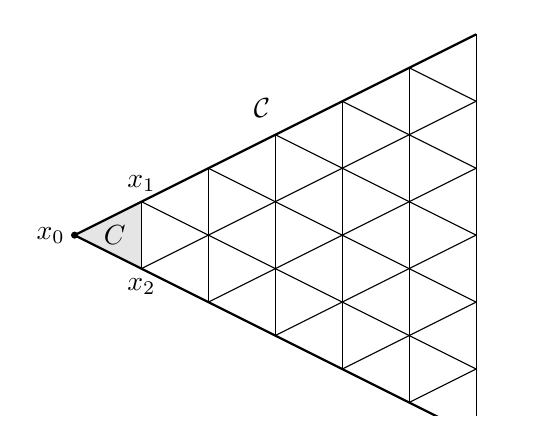
\begin{tikzpicture}[scale=0.85]
\clip(-0.7,-2.7) rectangle (6.5,3.1);
\fill[black!10](0,0)--(1,0.5)--(1,-0.5)--cycle;
\foreach \i in {1,...,6}{\draw[thin] (\i,{-0.5*\i})--(\i,{0.5*\i});}
\foreach \j in {0,...,5}{\draw[thin] (\j,{-0.5*\j})--(6,{3-\j});\draw[thin](\j,{0.5*\j})--(6,{-3+\j});}
\draw[thick](0,0)--(6,3) (0,0)--(6,-3);
\fill(0,0)circle(1.5pt)node[left]{$x_0$};
\node[above] at(1,0.5){$x_1$};\node[below]at(1,-0.5){$x_2$};
\node at(0.6,0){$C$};\node at(2.8,1.9){$\mathcal C$};
\end{tikzpicture}
\caption*{图1：特殊顶点、室与锥形室（据原书第140页重绘）。}
\end{figure}

$N(A)$ 中任意元素将公寓 $\mathcal A$ 保持为自身；它固定 $\mathcal A$ 的每一点，当且仅当属于 $^\circ M$。因此可将群 $W_1=N(A)/{}^\circ M$，即修正 Weyl 群（modified Weyl group），认同为 $\mathcal A$ 中的一个仿射线性变换群。$W_1$ 有两种半直积表示：

（a）令 $\Omega$ 为 $W_1$ 中将室 $C$ 保持为自身的元素组成的子群。$\mathcal A$ 中的墙（wall）为某些超平面，每面墙对应一个反射。这些反射生成 $W_1$ 的正规子群 $W_{\mathrm{aff}}$。由于 $W_{\mathrm{aff}}$ 在 $\mathcal A$ 的室集合上单可迁地作用，$W_1=\Omega\cdot W_{\mathrm{aff}}$ 为半直积。

（b）$W$ 中任意 $w$ 在 $K\cap N(A)$ 中有代表 $\omega(w)$，且 $^\circ M=K\cap M$。因此可将 $W=N(A)/M$ 与 $W_1$ 中 $x_0$ 的稳定子 $(K\cap N(A))/(K\cap M)$ 认同。$W_1$ 与 $\mathcal A$ 中平移群的交为 $M/{}^\circ M$，通过原书135页的正合列 (D) 将其与 $\Lambda$ 认同。于是 $W_1=W\cdot\Lambda$ 为半直积，$\Lambda$ 为正规子群。

现在可如下陈述基本结构定理。
\begin{originaltheorem}{Iwasawa 分解（Iwasawa decomposition）}
$G=PK$；更精确地，$G$ 为各集合 $P\omega(w)B$（$w$ 遍历 $W$）的不交并。
\end{originaltheorem}
\begin{originaltheorem}{Bruhat--Tits 分解（Bruhat--Tits decomposition）}
$G$ 为各集合 $Bw_1B$（$w_1$ 遍历修正 Weyl 群 $W_1$）的不交并。
\end{originaltheorem}
\begin{originaltheorem}{Cartan 分解（Cartan decomposition）}
令 $\Lambda^-$ 为 $\Lambda$ 中将 $\mathcal A$ 内与 $\mathcal C$ 相反的锥形室 $\mathcal C^-$ 映入自身的元素组成的子集。则 $G$ 为各集合 $K\operatorname{ord}_M^{-1}(\lambda)K$（$\lambda$ 遍历 $\Lambda^-$）的不交并。
\end{originaltheorem}
\begin{originaltheorem}{Iwahori 分解（Iwahori decomposition）}
$B=(B\cap N^-)(B\cap M)(B\cap N)$，且分解唯一。此外 $B\cap M={}^\circ M$，并且对满足 $\operatorname{ord}_M(m)\in\Lambda^-$ 的任意 $m\in M$，有
\[
m(B\cap N)m^{-1}\subseteq B\cap N,\qquad m^{-1}(B\cap N^-)m\subseteq B\cap N^-.
\]
\end{originaltheorem}
如前，以 $\Phi$ 表示 $G$ 关于 $A$ 的根系。将 $\Phi$ 的元素与 $\mathcal A$ 上仿射线性函数认同，使对 $\alpha\in\Phi,\lambda\in\Lambda$ 有 $\alpha(x_0+\lambda)=\langle\lambda,\alpha\rangle$。则锥形室 $\mathcal C$ 为满足对与抛物群 $P$ 相联系的基 $\Delta$ 中每个根 $\alpha$ 都有 $\alpha(x)>0$ 的点 $x\in\mathcal A$ 的集合。

以 $\Phi_0$ 表示在 $x_0$ 处为零且满足“超平面 $\alpha^{-1}(r)$ 为 $\mathcal A$ 中的墙，当且仅当实数 $r$ 是整数”的仿射线性函数 $\alpha$ 的集合。仿射根（affine root）是形如 $\alpha+k$ 的函数，其中 $\alpha\in\Phi_0,k\in\Z$；其集合记为 $\Phi_{\mathrm{aff}}$。对任意仿射根 $\alpha$，以 $S_\alpha$ 表示关于墙 $\alpha^{-1}(0)$ 的反射。$\alpha$ 遍历 $\Phi_0$（分别地，$\Phi_{\mathrm{aff}}$）时，各反射 $S_\alpha$ 生成群 $W$（分别地，$W_{\mathrm{aff}}$）。对 $\alpha\in\Phi_0$，存在唯一向量 $t_\alpha\in\Lambda$，使
\[
S_\alpha(x)=x-\alpha(x)t_\alpha,\qquad x\in\mathcal A.\tag{20}
\]
以 $a_\alpha$ 表示满足 $t_\alpha=\operatorname{ord}_M(a_\alpha)$ 的 $M$ 中任意元素。集合 $\Phi_1$ 由 $\Phi_0$ 添加那些满足 $(B\omega(S_\alpha)B:B)\ne\delta(a_\alpha)^{-1/2}$ 的 $\alpha\in\Phi_0$ 所对应的函数 $\alpha/2$ 得到。

$\Phi,\Phi_0,\Phi_1$ 均为通常意义下的根系（例如见 [37，第14页及以下]）。当 $G$ 分裂时，三者相同。在非分裂情形，只能断言：对任意 $\alpha\in\Phi$，$\Phi_0$ 中存在唯一与 $\alpha$ 成比例的根 $\lambda(\alpha)$，且约化根系 $\Phi_0$ 中每个元素都对适当 $\alpha\in\Phi$ 形如 $\lambda(\alpha)$。

令 $w_1\in W_1$。由于 $w_1$ 为模 $B$ 的子群 $^\circ M$ 的陪集，集合 $Bw_1B$ 为模 $B$ 的双陪集。令
\[
q(w_1)=(Bw_1B:B).\tag{21}
\]
由于 $K=BWB$，有
\[
(K:B)=\sum_{w\in W}q(w).\tag{22}
\]
令 $\Delta_1$ 为 $\mathcal A$ 中在室 $C$ 上为正且零集为 $C$ 的一面墙的仿射根集合。群 $W_1$ 由 $\Omega$ 和 $\alpha\in\Delta_1$ 的反射 $S_\alpha$ 生成。$q(w_1)$ 由
\[
q(w_1)=q(S_{\alpha_1})\cdots q(S_{\alpha_m})\tag{23}
\]
给出，其中 $w_1=\omega S_{\alpha_1}\cdots S_{\alpha_m}$ 为长度最小的分解，其长度为 $m$（$\omega\in\Omega,\alpha_1,\ldots,\alpha_m\in\Delta_1$）。

给每个 $\beta\in\Phi_1$ 赋予实数 $q_\beta>0$，由下述性质刻画：
\[
q_{w\beta}=q_\beta,\qquad\beta\in\Phi_1,w\in W;\tag{24a}
\]
\[
q(w)=\prod_{\beta>0,\ w^{-1}\beta<0}q_\beta;\tag{24b}
\]
\[
\delta(m)=\prod_{\beta>0}q_\beta^{-\beta(mx_0)},\qquad m\in M.\tag{24c}
\]
这些公式中 $\beta$ 遍历 $\Phi_1$，$\beta>0$ 指 $\beta$ 在 $\mathcal C$ 上只取正值。约定：若 $\alpha\in\Phi_0$ 但 $\alpha/2\notin\Phi_1$，则 $q_{\alpha/2}=1$。上述关系还有两个直接推论：
\[
q(S_\alpha)=q_\alpha q_{\alpha/2},\tag{24d}
\]
\[
\delta(a_\alpha)=q_\alpha^{-2}q_{\alpha/2}^{-1},\tag{24e}
\]
对任意 $\alpha\in\Phi_0,\alpha>0$ 成立。当 $G$ 分裂时，对每个根 $\beta\in\Phi=\Phi_0=\Phi_1$，$q_\beta$ 等于剩余域 $\mathfrak O_F/\mathfrak p_F$ 的阶 $q$。

Hecke 代数 $\mathcal H(G,B)$ 的结构已由 Iwahori 与 Matsumoto [30]、[31] 描述。
\begin{originaltheorem}{定理 3.6（Theorem 3.6）}
对 $w_1\in W_1$，令 $C(w_1)$ 为双陪集 $Bw_1B$ 的示性函数。

（a）族 $\{C(w_1)\}_{w_1\in W_1}$ 为复向量空间 $\mathcal H(G,B)$ 的一组基（Bruhat--Tits 分解！）。

（b）设 $w_1\in W_1$，且 $w_1=\omega S_{\alpha_1}\cdots S_{\alpha_m}$（$\omega\in\Omega,\alpha_i\in\Delta_1$）为最短长度 $m$ 的分解，则
\[
C(w_1)=C(\omega)C(S_{\alpha_1})\cdots C(S_{\alpha_m}).\tag{25}
\]
（c）对每个 $\alpha\in\Delta_1$，
\[
(C(S_\alpha)-1)(C(S_\alpha)+q(S_\alpha))=0,\tag{26}
\]
其中 $q(S_\alpha)$ 由上述 (21) 定义。\footnote{\textbf{译者注（本次校订）：}若 $C(S_\alpha)$ 是双陪集的示性函数，并归一化 Haar 测度使 $\mu(B)=1$，二次关系应为 $(C(S_\alpha)+1)(C(S_\alpha)-q(S_\alpha))=0$，即 $C(S_\alpha)^2=(q(S_\alpha)-1)C(S_\alpha)+q(S_\alpha)1$。原式 (26) 的两个符号颠倒了；例如在平凡表示上 $C(S_\alpha)$ 作用为标量 $q(S_\alpha)$，直接代入即可检验。若未作这一测度归一化，则应先将各示性函数除以 $\mu(B)$。}

（d）若 $\alpha,\beta$ 为 $\Delta_1$ 中不同元素，则存在整数 $m_{\alpha\beta}\geq2$，使
\[
\underbrace{C(S_\alpha)C(S_\beta)C(S_\alpha)\cdots}_{m_{\alpha\beta}\text{ 个因子}}
=\underbrace{C(S_\beta)C(S_\alpha)C(S_\beta)\cdots}_{m_{\alpha\beta}\text{ 个因子}}.\tag{27}
\]
此外，(26)、(27) 是各 $C(S_\alpha)$ 之间的一组完备关系。
\end{originaltheorem}
\origsubsection{3.6}{Iwahori 子群在表示上的作用}
本小节的主要结果由 Casselman [18] 和 Borel [4] 得到。
\begin{originaltheorem}{定理 3.7（Theorem 3.7）}
设 $(\pi,V)$ 为 $G$ 的任意容许表示。自然投影 $V\to V_N$ 定义从 $V^B$ 到 $(V_N)^{{}^\circ M}$ 的同构。
\end{originaltheorem}
首先用 $B$ 的 Iwahori 分解和定理2.3 证明中使用的方法，证明 $V^B$ 满射到 $(V_N)^{{}^\circ M}$。因为 $P$ 为极小抛物子群，论证有所简化。

为证明单射性，先证明：对给定 $v\in V(N)\cap V^B$，存在实数 $\varepsilon>0$，使对满足 $|\alpha(a)|_F\leq\varepsilon$（只要 $\alpha\in\Phi$ 在 $P$ 上为正）的每个 $a\in A$，有 $\pi(C(a))v=0$。由于定理3.6 中 $q(S_\alpha)>0$，该关系蕴含 $v=0$。
\begin{originaltheorem}{推论 3.4（Corollary 3.4）}
给定 $M$ 的任意非分歧特征 $\chi$，有直和分解 $I(\chi)=I(\chi)^B\oplus I(\chi)(N)$。
\end{originaltheorem}
因为 $^\circ M$ 在 $I(\chi)_N$ 上平凡作用，这是定理3.7 的推论。也可利用定理3.5 证明中的方法直接证明。

将 $G$ 分解成两两不交的开子集 $P\omega(w)B$（$w\in W$），容易得到 $I(\chi)^B$ 的一组基。事实上，$\omega(w)$ 正规化 $M$，且 $B\cap M={}^\circ M$ 包含于 $\chi\delta^{1/2}$ 的核，故下列函数在 $G$ 上定义良好：
\[
\Phi_{w,\chi}(g)=\begin{cases}\delta^{1/2}(m)\chi(m),&g=mn\omega(w)b,\\0,&g\notin P\omega(w)B.\end{cases}\tag{28}
\]
族 $\{\Phi_{w,\chi}\}_{w\in W}$ 即所求的基。

下一个结果归功于 Casselman [18]（另见 Borel [4]）。
\begin{originaltheorem}{定理 3.8（Theorem 3.8）}
设 $(\pi,V)$ 为 $G$ 的任意容许不可约表示。下列断言等价：

（a）$V$ 中有非零的 $B$ 不变向量，即 $V^B\ne0$；

（b）存在 $M$ 的某个非分歧特征 $\chi$，使 $(\pi,V)$ 同构于 $(\nu_\chi,I(\chi))$ 的子表示。
\end{originaltheorem}
由定理3.7，（a）意谓 $(V_N)^{{}^\circ M}\ne0$；由 Frobenius 互反律（定理3.4），（b）意谓 $V_N$ 的对偶空间中存在一个非零向量，在 $^\circ M$ 下不变并为群 $M$ 的特征向量。由于 $^\circ M$ 紧，在 $V_N$ 上连续作用，且 $M/{}^\circ M$ 交换，等价性立即成立。
\begin{originaltheorem}{推论 3.5（Corollary 3.5）}
设 $\chi$ 为 $M$ 的任意非分歧特征。空间 $I(\chi)^B$ 生成 $G$ 模 $I(\chi)$。
\end{originaltheorem}
用反证法。假设 $I(\chi)^B$ 不生成 $I(\chi)$。由于 $I(\chi)$ 有限生成，存在 $G$ 的不可约容许表示 $(\pi,V)$ 及非零 $G$ 同态 $u:I(\chi)\to V$，其核包含 $I(\chi)^B$。由于 $B$ 紧，$V^B=u(I(\chi)^B)=0$。对偶后得到单射的 $G$ 同态 $\widetilde u:\widetilde V\to I(\chi)^\sim$。由定理3.2，$I(\chi)^\sim\cong I(\chi^{-1})$；由定理3.8，$\widetilde V^B\ne0$。但有限维空间 $V^B,\widetilde V^B$ 彼此对偶，显然不可能。
\origsubsection{3.7}{交织算子（Intertwining operators）}
本小节假定非分歧特征 $\chi$ 正则，即 $w$ 遍历 $W$ 时各 $w\chi$ 互异。

推论3.2 可改述为：给定 $w\in W$，$I(\chi)$ 上存在非零线性形式 $L_w$，使
\[
L_w(\nu_\chi(mn)f)=\delta^{1/2}(m)(w\chi)(m)L_w(f),\quad m\in M,n\in N,f\in I(\chi),\tag{29}
\]
且在相差常数倍意义下唯一。对支集不与 $F_r$ 相交的函数 $f$（$r=d(w^{-1})$），用
\[
L_w(f)=\int_{N(w)\backslash N}f(\omega(w)^{-1}n)\,d\bar n\tag{30}
\]
归一化 $L_w$。Haar 测度选得使 $N(w)\backslash N(w)(N\cap B)$ 的测度为 $1$。由 $L_w$ 定义交织算子 $T_w:I(\chi)\to I(w\chi)$：
\[
T_wf(g)=L_w(\nu_\chi(g)f),\quad f\in I(\chi),g\in G.\tag{31}
\]
容易验证 $L_w$，从而 $T_w$，只依赖于 $w$，不依赖于所选代表 $\omega(w)$。

由 Iwasawa 分解 $G=PK$，而 $M$ 的特征 $\delta^{1/2}\chi$ 在 $M\cap K={}^\circ M$ 上平凡，$I(\chi)$ 中存在唯一在 $K$ 下不变且满足 $\Phi_{K,\chi}(1)=1$ 的函数 $\Phi_{K,\chi}$。具体地，
\[
\Phi_{K,\chi}(mnk)=\delta^{1/2}(m)\chi(m),\quad m\in M,n\in N,k\in K.\tag{32}
\]
若 $M,N$ 上 Haar 测度按 $\int_{M\cap K}dm=\int_{N\cap K}dn=1$ 归一化，也可将 $\Phi_{K,\chi}$ 定义为 $P_\chi(I_K)$，其中 $P_\chi$ 如原书136页定义，$I_K$ 是 $K$ 的示性函数。空间 $I(\chi)^K$ 由 $\Phi_{K,\chi}$ 的常数倍组成。

下述定理同样归功于 Casselman [18]。
\begin{originaltheorem}{定理 3.9（Theorem 3.9）}
算子 $T_w$ 将 $I(\chi)^K$ 映入 $I(w\chi)^K$。更精确地，
\[
T_w(\Phi_{K,\chi})=c_w(\chi)\Phi_{K,w\chi},\tag{33}
\]
其中常数 $c_w(\chi)$ 定义为
\[
c_w(\chi)=\prod_\alpha c_\alpha(\chi),\tag{34}
\]
\[
c_\alpha(\chi)=\frac{(1-q_{\alpha/2}^{-1/2}q_\alpha^{-1}\chi(a_\alpha))(1+q_{\alpha/2}^{-1/2}\chi(a_\alpha))}{1-\chi(a_\alpha)^2}.\tag{35}
\]
(34) 的乘积遍历 $\Phi_0$ 中在 $\mathcal C$ 上为正而 $w\alpha$ 在 $\mathcal C$ 上为负的仿射根 $\alpha$。
\end{originaltheorem}
当 $G$ 分裂，(35) 简化为
\[
c_\alpha(\chi)=\frac{1-q^{-1}\chi(a_\alpha)}{1-\chi(a_\alpha)}.\tag{36}
\]
证明定理3.9 的关键在于处理 $w$ 是 $\Phi_0$ 中某个单根 $\beta$ 对应的反射的情形。此时 $\Phi_0$ 中恰有一个正根 $\alpha$ 被 $w$ 映为负根，即 $\alpha=\beta$。一般情形随即成立，因为当 $w_1,w_2$ 的长度之和等于 $w_1w_2$ 的长度时，$T_{w_1w_2}=T_{w_1}T_{w_2}$。
\begin{originaltheorem}{推论 3.6（Corollary 3.6）}
交织映射 $T_w$ 是 $I(\chi)$ 到 $I(w\chi)$ 的同构，当且仅当 $c_w(\chi),c_{w^{-1}}(w\chi)$ 均非零。
\end{originaltheorem}
事实上，由定理3.9，$T_{w^{-1}}T_w$ 为乘以 $c_w(\chi)c_{w^{-1}}(w\chi)$ 的标量算子。

由此可加强定理3.3 中的不可约性判据：
\begin{originaltheorem}{定理 3.10（Theorem 3.10）}
设 $\chi$ 为 $M$ 的任意非分歧正则特征，则 $G$ 的表示 $(\nu_\chi,I(\chi))$ 不可约，当且仅当对 $\Phi_0$ 中在 $\mathcal C$ 上为正的每个正根 $\alpha$，$c_\alpha(\chi)\ne0,c_\alpha(w_0\chi)\ne0$，其中 $w_0$ 是 $W$ 中将 $\mathcal C$ 映到 $\mathcal C^-$ 的唯一元素。
\end{originaltheorem}
\origsection{IV}{球面函数（Spherical functions）}
\origsubsection{4.1}{一些积分公式（Some integration formulas）}
沿用上一部分的记号。若 $\Gamma$ 是群 $G,M,N,K$ 中任意一个，则 $\Gamma$ 幺模。按 $\int_{\Gamma\cap K}d\gamma=1$ 归一化其左右不变 Haar 测度。群 $P=MN$ 非幺模。直接检验可知，公式
\[
\int_P f(p)\,d_lp=\int_M\int_N f(mn)\,dm\,dn,\tag{1}
\]
\[
\int_P f(p)\,d_rp=\int_M\int_N f(nm)\,dm\,dn,\tag{2}
\]
分别定义 $P$ 上左不变 Haar 测度 $d_lp$ 和右不变 Haar 测度 $d_rp$。由于 $^\circ M=M\cap K$ 是 $M$ 的最大紧子群，有 $P\cap K=(M\cap K)(N\cap K)$，因此
\[
\int_{P\cap K}d_lp=\int_{P\cap K}d_rp=1.\tag{3}
\]
Haar 测度与 Iwasawa 分解由下列公式联系：
\[
\int_G f(g)\,dg=\int_K\int_Pf(pk)\,dk\,d_lp,\tag{4}
\]
\[
\int_G f(g)\,dg=\int_K\int_Pf(kp)\,dk\,d_rp,\qquad f\in C_c(G).\tag{5}
\]
例如证明 (4)。通过规则
\[
u_h(pk^{-1})=\int_{P\cap K}h(kp_1,pp_1)\,d_lp_1\tag{6}
\]
定义线性映射 $h\mapsto u_h:C_c(K\times P)\to C_c(G)$。则 $C_c(K\times P)$ 上的线性形式 $h\mapsto\int_Gu_h(g)\,dg$ 为 $K\times P$ 上左不变 Haar 测度。根据归一化，有
\[
\int_Gu_h(g)\,dg=\int_K\int_Ph(k,p)\,dk\,d_lp.\tag{7}
\]
在 (6)、(7) 中取 $h(k,p)=f(pk^{-1})$，即得 (4)。

由 $\delta$ 的定义（见原书135页），对任意 $f\in C_c(N)$ 有
\[
\int_Nf(mnm^{-1})\,dn=\delta(m)^{-1}\int_Nf(n)\,dn.\tag{8}
\]
从而得到 $P$ 上 Haar 测度的另一些表达式：
\[
\int_Pf(p)\,d_lp=\int_M\int_N\delta(m)^{-1}f(nm)\,dm\,dn,\tag{9}
\]
\[
\int_Pf(p)\,d_rp=\int_M\int_N\delta(m)f(mn)\,dm\,dn.\tag{10}
\]
换言之，$P$ 的模函数为
\[
\Delta_P(mn)=\delta(m)^{-1},\qquad m\in M,n\in N.\tag{11}
\]
群 $N$ 幺幂，$M$ 通过内自同构作用于 $N$。容易构造 $N$ 的子群列 $N=N_0\supseteq N_1\supseteq\cdots\supseteq N_{r-1}\supseteq N_r=1$，各项均在 $M$ 下不变，且对 $j=1,\ldots,r$，$N_{j-1}/N_j$ 同构于某个 $F$ 向量空间，$M$ 在其上线性作用。对 $m\in M$ 令
\[
\Delta(m)=|\det(\Ad_{\mathfrak n}(m)-1_{\mathfrak n})|_F,\tag{12}
\]
对 $r$ 归纳得到积分公式
\[
\int_Nf(n)\,dn=\Delta(m)\int_Nf(nmn^{-1}m^{-1})\,dn,\tag{13}
\]
适用于 $f\in C_c(N)$ 和满足 $\Delta(m)\ne0$ 的任意 $m\in M$（见 [28，引理22]）。

现在定义所谓轨道积分（orbital integral）。设 $m\in M$ 满足 $\Delta(m)\ne0$，令 $Z(m)$ 为 $m$ 在 $G$ 中的中心化子，$G_m$ 为其共轭类。则 $A\subseteq M$，$Z(m)\cap M$ 在 $Z(m)$ 中指数有限；由于 $M/A$ 紧，$Z(m)/A$ 亦紧。此外，共轭类 $G_m$ 在 $G$ 中闭，故映射 $gZ(m)\mapsto gmg^{-1}$ 为 $G/Z(m)$ 到 $G_m$ 的同胚。因此映射 $gA\mapsto gmg^{-1}:G/A\to G$ 为固有映射（proper map），可以遵循 Harish-Chandra，对任意 $f\in C_c(G)$ 令
\[
F_f(m)=\Delta(m)\int_{G/A}f(gmg^{-1})\,d\bar g.\tag{14}
\]
$A$ 上 Haar 测度归一化为 $\int_{M/A}d\bar m=1$。
\begin{originaltheorem}{引理 4.1（Lemma 4.1）}
设 $f\in\mathcal H(G,K)$，$m\in M$ 且 $\Delta(m)\ne0$，则 $F_f(m)=\int_Nf(nm)\,dn$。
\end{originaltheorem}
由 (2)、(5)，对在 $K$ 左平移下不变的任意 $u\in C_c(G)$，有
\[
\int_Gu(g)\,dg=\int_M\int_Nu(nm_1)\,dm_1\,dn.\tag{15}
\]
令 $u(g)=f(gmg^{-1})$，得到
\[
F_f(m)=\int_{M/A}h(m_1)\,d\bar m_1,\tag{16}
\]
\[
h(m_1)=\Delta(m)\int_Nf(nm_1mm_1^{-1}n^{-1})\,dn.\tag{17}
\]
固定 $m_1$，令 $m_2=m_1mm_1^{-1}$。由 (12)，$\Delta(m)=\Delta(m_2)$，所以
\[
\begin{aligned}
h(m_1)&=\Delta(m_2)\int_Nf((nm_2n^{-1}m_2^{-1})m_2)\,dn&&\text{由 (17)}\\
&=\int_Nf(nm_2)\,dn&&\text{由 (13)}.
\end{aligned}
\]
注意 $M/{}^\circ M=M/(M\cap K)$ 交换，所以 $m_2\in mK$。$f$ 在 $K$ 的右平移下不变，故对每个 $n\in N$，$f(nm_2)=f(nm)$。因此对任意 $m_1\in M$，$h(m_1)=\int_Nf(nm)\,dn$。因为 $M/A$ 的测度为 $1$，由 (16) 得引理4.1。
\origsubsection{4.2}{Satake 同构（Satake isomorphism）}
下面介绍 Satake [38] 的构造。它对应于 Harish-Chandra 在实 Lie 群理论中的一个经典构造。

对任意 $\lambda\in\Lambda$，令 $\operatorname{ch}(\lambda)$ 为 $M$ 的子集 $\operatorname{ord}_M^{-1}(\lambda)$ 的示性函数。由于 $\int_{M\cap K}dm=1$，有
\[
\operatorname{ch}(\lambda)*\operatorname{ch}(\lambda')=\operatorname{ch}(\lambda+\lambda'),\qquad\lambda,\lambda'\in\Lambda.\tag{18}
\]
各 $\operatorname{ch}(\lambda)$ 构成复代数 $\mathcal H(M,{}^\circ M)$ 的一组基，因此后者可与群代数 $\C[\Lambda]$ 认同。

用公式
\[
Sf(m)=\delta(m)^{1/2}\int_Nf(mn)\,dn=\delta(m)^{-1/2}\int_Nf(nm)\,dn\tag{19}
\]
定义线性映射 $S:\mathcal H(G,K)\to\mathcal H(M,{}^\circ M)$，其中 $f\in\mathcal H(G,K),m\in M$。两个积分由 (8) 相等。显然 $Sf\in C_c(M)$；由于 $f$ 在 $K$ 下双不变，$^\circ M=M\cap K$，$Sf$ 在 $^\circ M$ 下也双不变。

下述基本定理归功于 Satake [38]。
\begin{originaltheorem}{定理 4.1（Theorem 4.1）}
Satake 变换（Satake transformation）$S$ 为从 $\mathcal H(G,K)$ 到 $\C[\Lambda]$ 中 Weyl 群 $W$ 不变量构成的子代数 $\C[\Lambda]^W$ 的代数同构。
\end{originaltheorem}
证明的主要步骤如下。

（A）$S$ 是代数同态。由构造，$S$ 为三个线性映射的复合：
\[
\mathcal H(G,K)\xrightarrow\alpha\mathcal H(P)\xrightarrow\beta\mathcal H(M)\xrightarrow\gamma\mathcal H(M).
\]
这里 $\alpha$ 仅为函数从 $G$ 到 $P$ 的限制，由 (4) 的一个简单推论可知它与卷积相容。$\beta$ 为 $(\beta u)(m)=\int_Nu(mn)\,dn$，容易验证与卷积相容。$\gamma$ 为 $(\gamma f)(m)=f(m)\delta(m)^{1/2}$；因为 $\delta$ 是 $M$ 的特征，也与卷积相容。

（B）$S$ 的像包含于 $\C[\Lambda]^W$。由于 $W=(N(A)\cap K)/{}^\circ M$，此性质等价于
\[
Sf(xmx^{-1})=Sf(m),\qquad m\in M,x\in N(A)\cap K.\tag{20}
\]
函数 $m\mapsto\det(\Ad_{\mathfrak n}(m)-1_{\mathfrak n})$ 从 $M$ 到 $F$ 为非零多项式。因此使该函数非零的 $M$ 中元素稠密，称为正则元素。由连续性，只需对正则 $m$ 证明 (20)。由引理4.1，对 $M$ 中正则 $m$，
\[
Sf(m)=D(m)\int_{G/A}f(gmg^{-1})\,d\bar g,\tag{21}
\]
其中 $D(m)=\Delta(m)\delta(m)^{-1/2}$。因此
\[
\begin{aligned}
D(m)^2&=|\det(\Ad_{\mathfrak n}(m)-1_{\mathfrak n})|_F^2|\det\Ad_{\mathfrak n}(m)|_F^{-1}\\
&=|\det(\Ad_{\mathfrak n}(m)-1_{\mathfrak n})|_F|\det(\Ad_{\mathfrak n}(m^{-1})-1_{\mathfrak n})|_F\\
&=|\det(\Ad_{\mathfrak n}(m)-1_{\mathfrak n})|_F|\det(\Ad_{\mathfrak n^-}(m)-1_{\mathfrak n^-})|_F.
\end{aligned}
\]
最后一个等号，例如可由 $M$ 的任意极大环面在 $\mathfrak n\otimes_F\overline F$ 与 $\mathfrak n^-\otimes_F\overline F$ 中的权互为逆得到，$\overline F$ 为 $F$ 的代数闭包。由于 $\mathfrak g=\mathfrak n\oplus\mathfrak m\oplus\mathfrak n^-$，有
\[
D(m)=|\det(\Ad_{\mathfrak g/\mathfrak m}(m)-1_{\mathfrak g/\mathfrak m})|_F^{1/2},\tag{22}
\]
因而
\[
D(xmx^{-1})=D(m),\qquad m\in M,x\in N(A).\tag{23}
\]
另一方面，紧群 $N(A)\cap K$ 通过内自同构作用于 $G,A$，故保持二者 Haar 测度，从而保持 $G/A$ 上的 $G$ 不变测度。设 $m\in M$ 正则，$x\in N(A)\cap K$，$f\in\mathcal H(G,K)$。对任意 $g\in G$，$f(xgx^{-1})=f(g)$，故
\[
\begin{aligned}
\int_{G/A}f(g(xmx^{-1})g^{-1})\,d\bar g
&=\int_{G/A}f((x^{-1}gx)m(x^{-1}gx)^{-1})\,d\bar g\\
&=\int_{G/A}f(gmg^{-1})\,d\bar g.
\end{aligned}
\]
结合 (21)、(23) 与刚得到的积分不变性，便得 (20)。

（C）线性映射 $S:\mathcal H(G,K)\to\C[\Lambda]^W$ 为双射。仍令 $\Lambda^-$ 为 $\Lambda$ 中将 $\mathcal C^-$ 映入自身的平移。对 $\lambda\in\Lambda^-$，令 $\varphi_\lambda$ 为双陪集 $K\operatorname{ord}_M^{-1}(\lambda)K$ 的示性函数。由 Cartan 分解，族 $\{\varphi_\lambda\}_{\lambda\in\Lambda^-}$ 为 $\mathcal H(G,K)$ 的一组基。此外，$\Lambda$ 中任意元素在 $W$ 下共轭于 $\Lambda^-$ 的唯一元素。于是令
\[
\operatorname{ch}'(\lambda)=\frac1{|W(\lambda)|}\sum_{w\in W}\operatorname{ch}(w\lambda),\tag{24}
\]
得到 $\C[\Lambda]^W$ 的一组基，其中 $W(\lambda)$ 为 $\lambda$ 在 $W$ 中的稳定子。用
\[
S\varphi_{\lambda'}=\sum_\lambda c(\lambda,\lambda')\operatorname{ch}'(\lambda)\tag{25}
\]
定义矩阵 $\{c(\lambda,\lambda')\}$，$\lambda,\lambda'$ 遍历 $\Lambda^-$。

为计算这些系数，在 $M$ 中分别选取 $\lambda,\lambda'$ 的代表 $m,m'$。则（$\mu$ 是 $G$ 上 Haar 测度）
\[
c(\lambda,\lambda')=S\varphi_{\lambda'}(m)=\delta(m)^{-1/2}\mu(Km'K\cap NmK).\tag{26}
\]
显然 $KmK\cap NmK\supseteq mK$，故
\[
c(\lambda,\lambda)\geq\delta(m)^{-1/2}.\tag{27}
\]
而且除非 $\lambda'-\lambda$ 为正根以非负实系数的线性组合，否则 $Km'K\cap NmK$ 为空。采用适当字典序 $\geq$，得到除非 $0\geq\lambda'\geq\lambda$，否则 $c(\lambda,\lambda')=0$。由 (27)，$c(\lambda,\lambda)\ne0$，故各 $S\varphi_{\lambda'}$ 构成 $\C[\Lambda]^W$ 的一组基，（C）得证。
\begin{originaltheorem}{推论 4.1（Corollary 4.1）}
代数 $\mathcal H(G,K)$ 交换，且作为复代数有限生成。
\end{originaltheorem}
代数 $\C[\Lambda]$ 交换，若 $\{\lambda_1,\ldots,\lambda_m\}$ 为 $\Lambda$ 的一组 $\Z$ 基，则它由 $\operatorname{ch}(\lambda_i)$ 与 $\operatorname{ch}(\lambda_i^{-1})$（$1\le i\le m$）生成。由于 $W$ 有限，由交换代数的熟知结果，\footnote{例如见 N. Bourbaki, \emph{Commutative algebra}, Chapter V, p. 323, Addison-Wesley, 1972。}$\C[\Lambda]^W$ 为有限生成复代数，且 $\C[\Lambda]$ 为其上的有限生成模。

接下来确定从 $\mathcal H(G,K)$ 到 $\C$ 的代数同态。设 $\chi$ 为 $M$ 的任意非分歧特征。由于 $\int_{{}^\circ M}dm=1$，映射 $f\mapsto\int_Mf(m)\chi(m)\,dm$ 为 $\mathcal H(M,{}^\circ M)$ 到 $\C$ 的含幺同态（unitary homomorphism），全部这样的同态均以此得到。用
\[
\omega_\chi(f)=\int_MSf(m)\chi(m)\,dm\tag{28}
\]
定义线性映射 $\omega_\chi:\mathcal H(G,K)\to\C$。
\begin{originaltheorem}{推论 4.2（Corollary 4.2）}
从 $\mathcal H(G,K)$ 到 $\C$ 的任意含幺同态，都对 $M$ 的某个非分歧特征 $\chi$ 形如 $\omega_\chi$。此外，$\omega_\chi=\omega_{\chi'}$ 当且仅当存在 $w\in W$，使 $\chi'=w\chi$。
\end{originaltheorem}
此推论来自定理4.1 及有限群作用于多项式代数时不变量的经典性质（见上一脚注）。换言之，从 $\mathcal H(G,K)$ 到 $\C$ 的含幺同态集合，与非分歧特征集 $X$ 中 $W$ 的轨道集 $X/W$ 一一对应。关于 $X/W$ 的讨论见3.2。由于 $X$ 同构于满足 $X^*(T)=\Lambda$ 的复环面 $T$，$X/W$ 为复仿射代数簇（affine algebraic variety），Satake 同构给出 $\mathcal H(G,K)$ 与 $X/W$ 上多项式函数代数的同构。
\origsubsection{4.3}{球面函数的确定（Determination of the spherical functions）}
由于双陪集 $KgK$ 的示性函数构成复向量空间 $\mathcal H(G,K)$ 的一组基，可如下定义其对偶空间与 $G$ 上 $K$ 双不变函数空间的同构：
\[
\omega(f)=\int_G f(g)\Gamma(g)\,dg,\qquad f\in\mathcal H(G,K),\tag{29}
\]
\[
\Gamma(g)=\omega(I_{KgK})\big/\int_{KgK}dg_1,\qquad g\in G.\tag{30}
\]
断言下列条件等价：\footnote{\textbf{译者注（本次校订）：}以下等价性需要归一化条件 $\Gamma(1)=1$，这也是随后定义4.1采用的条件。若不加归一化，一个球面函数的任意非零常数倍仍满足 (c)，却通常不满足 (a)、(b)。}
\begin{enumerate}
\item[(a)] $\omega$ 是从 $\mathcal H(G,K)$ 到 $\C$ 的代数同态；
\item[(b)] 对 $g_1,g_2\in G$ 有
\[
\Gamma(g_1)\Gamma(g_2)=\int_K\Gamma(g_1kg_2)\,dk;\tag{31}
\]
\item[(c)] 对任意 $f\in\mathcal H(G,K)$，存在常数 $\lambda(f)$，使
\[
f*\Gamma=\Gamma*f=\lambda(f)\Gamma.\tag{32}
\]
\end{enumerate}
（a）、（b）的等价性由下列计算
\[
\begin{aligned}
\omega(f_1*f_2)&=\iint\Gamma(g_1g_2)f_1(g_1)f_2(g_2)\,dg_1\,dg_2\\
&=\int_G f_1(g_1)\,dg_1\int_Gf_2(g_2)\,dg_2\int_K\Gamma(g_1kg_2)\,dk
\end{aligned}
\]
及 $G\times G$ 上的函数 $(g_1,g_2)\mapsto\int_K\Gamma(g_1kg_2)\,dk$ 在 $K\times K$ 的左右平移下不变的事实得到。

（a）、（c）的等价性由公式
\[
\omega(f_1*f_2)=\int f_2(g)(\check f_1*\Gamma)(g)\,dg
=\int f_1(g)(\Gamma*\check f_2)(g)\,dg
\]
得到，其中 $f_1,f_2\in\mathcal H(G,K)$，$\check f(g)=f(g^{-1})$。所以 $\lambda(f)=\omega(\check f)$。
\begin{originaltheorem}{定义 4.1（Definition 4.1）}
$G$ 上关于 $K$ 的（带状）球面函数（zonal spherical function）为 $G$ 上的一个 $K$ 双不变函数 $\Gamma$，满足 $\Gamma(1)=1$ 以及上述等价性质（a）、（b）、（c）。
\end{originaltheorem}
下面用球面函数的语言重新表述前面的结果。设 $\chi$ 为 $M$ 的任意非分歧特征。回顾 $\Phi_{K,\chi}$ 由
\[
\Phi_{K,\chi}(mnk)=\chi(m)\delta^{1/2}(m),\qquad m\in M,n\in N,k\in K,\tag{33}
\]
定义。令
\[
\Gamma_\chi(g)=\int_K\Phi_{K,\chi}(kg)\,dk,\qquad g\in G.\tag{34}
\]
\begin{originaltheorem}{定理 4.2（Theorem 4.2）}
（a）$G$ 上关于 $K$ 的球面函数正是各 $\Gamma_\chi$。

（b）设 $\chi,\chi'$ 为 $M$ 的非分歧特征。球面函数 $\Gamma_\chi,\Gamma_{\chi'}$ 相等，当且仅当存在 $w\in W$，使 $\chi'=w\chi$。
\end{originaltheorem}
显然 $\Gamma_\chi$ 在 $K$ 下双不变，且 $\Gamma_\chi(1)=1$。由推论4.2 及公式
\[
\omega_\chi(f)=\int_G\Gamma_\chi(g)f(g)\,dg,\qquad f\in\mathcal H(G,K),\tag{35}
\]
得到定理4.2。后式证明如下：
\[
\begin{aligned}
\int_G\Gamma_\chi(g)f(g)\,dg
&=\int_G\Phi_{K,\chi}(g)f(g)\,dg\\
&=\int_K\int_M\int_N\Phi_{K,\chi}(mnk)f(mnk)\,dk\,dm\,dn\\
&=\int_M\chi(m)\delta(m)^{1/2}\,dm\int_Nf(mn)\,dn\\
&=\int_M\chi(m)Sf(m)\,dm=\omega_\chi(f).
\end{aligned}
\]
使用了积分关系 (1)、(4)。
\origsubsection{4.4}{球面主系列表示（The spherical principal series of representations）}
\begin{originaltheorem}{定义 4.2（Definition 4.2）}
$G$ 的表示若光滑、不可约，且包含非零的 $K$ 不变向量，就称为（关于 $K$ 的）球面表示（spherical representation）。
\end{originaltheorem}
设 $\Gamma$ 为 $G$ 上关于 $K$ 的球面函数。以 $V_\Gamma$ 表示 $G$ 上形如 $f(g)=\sum_{i=1}^n c_i\Gamma(gg_i)$ 的函数空间，其中 $c_i\in\C,g_i\in G$。由球面函数的函数方程 (31)，得
\[
\int_Kf(gkg')\,dk=\Gamma(g)f(g'),\qquad f\in V_\Gamma,g,g'\in G.\tag{36}
\]
令 $G$ 通过右平移作用在 $V_\Gamma$ 上：
\[
(\pi_\Gamma(g)f)(g_1)=f(g_1g),\qquad f\in V_\Gamma,g,g_1\in G.\tag{37}
\]
我们将证明 $(\pi_\Gamma,V_\Gamma)$ 是球面表示，并且 $V_\Gamma$ 中在 $\pi_\Gamma(K)$ 下不变的元素恰为 $\Gamma$ 的常数倍。事实上，对任意 $f\in V_\Gamma$，显然存在 $G$ 的紧开子群 $K_f$，使 $f$ 在 $K_f$ 的右平移下不变；故表示光滑。取非零 $f\in V_\Gamma$，选取 $g'\in G$ 使 $f(g')\ne0$。函数方程 (36) 可改写为
\[
\Gamma=f(g')^{-1}\int_K\pi_\Gamma(kg')f\,dk
=f(g')^{-1}\pi_\Gamma(I_{Kg'})f.\tag{38}
\]
因此，包含 $f$ 且在 $\pi_\Gamma(G)$ 下不变的任意向量子空间，都包含 $\Gamma$，因而等于 $V_\Gamma$。最后，若 $f\in V_\Gamma$ 在 $\pi_\Gamma(K)$ 下不变，在 (36) 中代入 $g'=1$ 得 $f=f(1)\Gamma$。
\begin{originaltheorem}{定理 4.3（Theorem 4.3）}
设 $(\pi,V)$ 是 $G$ 的任意球面表示。存在唯一球面函数 $\Gamma$，使 $(\pi,V)$ 同构于 $(\pi_\Gamma,V_\Gamma)$。
\end{originaltheorem}
仍以 $V^K$ 表示 $V$ 中的 $\pi(K)$ 不变向量子空间。对任意 $f\in\mathcal H(G,K)$，$\pi(f)$ 保持 $V^K$，故 $V^K$ 为 $\mathcal H(G,K)$ 模。它是一个单模。事实上，设 $v\ne0,v'\in V^K$。由于 $\mathcal H(G)$ 模 $V$ 为单模，存在 $f\in\mathcal H(G)$ 使 $v'=\pi(f)v$。函数 $f_K=I_K*f*I_K$ 属于 $\mathcal H(G,K)$，且 $v'=\pi(f_K)v$，故断言成立。

复代数 $\mathcal H(G,K)$ 交换且维数可数。用证明 Schur 引理的论证（见原书118页），或用 Hilbert 零点定理（Hilbert's Zero Theorem），可知其上的任意单模复维数为一。因此 $\dim_\C V^K=1$，并存在含幺同态 $\omega:\mathcal H(G,K)\to\C$，使
\[
\pi(f)v=\omega(f)v,\qquad f\in\mathcal H(G,K),v\in V^K.\tag{39}
\]
令 $(\widetilde\pi,\widetilde V)$ 为 $(\pi,V)$ 的逆反表示。$\widetilde V$ 中的 $K$ 不变向量空间 $\widetilde V^K$ 为 $V^K$ 的对偶，故亦为一维。选取 $v\in V^K,\widetilde v\in\widetilde V^K$ 使 $\langle\widetilde v,v\rangle=1$，用
\[
\Gamma(g)=\langle\widetilde v,\pi(g)v\rangle,\qquad g\in G,\tag{40}
\]
定义 $G$ 上函数。由 (39)、(40)，对任意 $f\in\mathcal H(G,K)$，$\omega(f)=\int_G\Gamma(g)f(g)\,dg$。显然 $\Gamma(1)=1$ 且 $\Gamma$ 在 $K$ 下双不变，所以是球面函数。

将任意 $v'\in V$ 映到系数 $\pi_{v',\widetilde v}$ 的映射，定义 $(\pi,V)$ 到 $(\pi_\Gamma,V_\Gamma)$ 的同构。此外，对于 $G$ 上任意球面函数 $\Gamma'$，$(\pi,V)$ 同构于 $(\pi_{\Gamma'},V_{\Gamma'})$，当且仅当
\[
\pi(I_K)\pi(g)\pi(I_K)=\Gamma'(g)\pi(I_K),\qquad g\in G.\tag{41}
\]
这仅对 $\Gamma'=\Gamma$ 成立。证毕。

球面函数定义和本节至此的结果，仅依赖于 $K$ 紧开且 $\mathcal H(G,K)$ 交换。现在使用定理4.2 给出的球面函数分类。设 $\chi$ 为 $M$ 的任意非分歧特征；当 $\Gamma=\Gamma_\chi$ 时，以 $(\pi_\chi,V_\chi)$ 代替 $(\pi_\Gamma,V_\Gamma)$。表示族 $\{(\pi_\chi,V_\chi)\}_{\chi\in X}$ 称为 $G$ 的球面主系列表示（spherical principal series）。

这一系列的主要性质如下，均可由前面的结果直接推出：
\begin{enumerate}
\item[(a)] 每个 $(\pi_\chi,V_\chi)$ 都不可约且容许，$V_\chi$ 中被 $\pi_\chi(K)$ 固定的函数恰为 $\Gamma_\chi$ 的常数倍。
\item[(b)] 设 $\chi,\chi'$ 为 $M$ 的非分歧特征。$(\pi_\chi,V_\chi)$ 与 $(\pi_{\chi'},V_{\chi'})$ 同构，当且仅当存在 $w\in W$ 使 $\chi'=w\chi$。
\item[(c)] 假定非分歧主系列中的 $(\nu_\chi,I(\chi))$ 不可约。对任意 $f\in I(\chi)$，定义 $f^\natural(g)=\int_K f(kg)\,dk$。则 $f\mapsto f^\natural$ 为 $(\nu_\chi,I(\chi))$ 与 $(\pi_\chi,V_\chi)$ 的同构。
\item[(d)] 一般地，设 $0=V_0\subseteq V_1\subseteq\cdots\subseteq V_{r-1}\subseteq V_r=I(\chi)$ 为 $\mathcal H(G)$ 模 $I(\chi)$ 的 Jordan--Hölder 列。存在唯一指标 $j$，$1\leq j\leq r$，使 $G$ 在 $V_j/V_{j-1}$ 中的表示为球面表示；它同构于 $(\pi_\chi,V_\chi)$。
\end{enumerate}
最后两项来自：$\Phi_{K,\chi}$ 在相差常数倍的意义下为 $I(\chi)$ 中唯一被 $\nu_\chi(K)$ 固定的函数，以及可写成 $\Gamma_\chi=\Phi_{K,\chi}^\natural$ 的关系 (34)。
\paragraph*{注}
（1）不借助 Satake 定理4.1，也容易证明只要 $(\nu_\chi,I(\chi))$ 不可约，它就是球面表示。此时对任意 $w\in W$，$(\nu_\chi,I(\chi))$ 与 $(\nu_{w\chi},I(w\chi))$ 等价，因此给出 Satake 定理步骤（B）的另一证明（见判据3.10，原书144页）。

（2）有界球面函数（bounded spherical function）的刻画见 Macdonald [37，第63页]；它们构成 $G$ 上 $K$ 双不变可积函数的 Banach 代数的谱。哪些球面函数为正定的（positive-definite），或者等价地，哪些球面表示预酉，似乎尚不清楚。
\origsubsection{4.5}{球面函数的显式公式}
下述结果归功于 Macdonald [36]、[37]。
\begin{originaltheorem}{定理 4.4（Theorem 4.4）}
假定 $M$ 的非分歧特征 $\chi$ 正则。对任意 $m\in M^-$，球面函数的值为
\[
\Gamma_\chi(m)=Q^{-1}\delta(m)^{1/2}\sum_{w\in W}\mathbf c(w\chi)(w\chi)(m),\tag{42}
\]
其中
\[
Q=\sum_{w\in W}q(w)^{-1},\tag{43}
\]
\[
\begin{aligned}
\mathbf c(\lambda)=\prod_{\alpha>0}&(1-q_{\alpha/2}^{-1/2}q_\alpha^{-1}\lambda(a_\alpha)^{-1})\\
&\cdot(1+q_{\alpha/2}^{-1/2}\lambda(a_\alpha)^{-1})(1-\lambda(a_\alpha)^{-2})^{-1}
\end{aligned}\tag{44}
\]
适用于 $M$ 的任意正则非分歧特征 $\lambda$，乘积遍历 $\Phi_0$ 中在锥形室 $\mathcal C$ 上为正的根 $\alpha$。
\end{originaltheorem}
下面概述 Casselman [18] 的证明；其主要依据是交织算子的性质。使用3.7 的记号。

对每个 $w\in W$，$I(\chi)$ 上线性形式 $L_w$ 在 $M$ 下按特征 $\delta^{1/2}(w\chi)$ 变换，且在 $I(\chi)(N)$ 上为零。由于 $\chi$ 正则，这些特征互异，因而 $L_w$ 线性无关。向量空间 $I(\chi)^B$ 与 $I(\chi)(N)$ 在 $I(\chi)$ 中互补，且维数为 $|W|$。所以 $I(\chi)^B$ 中存在由
\[
L_w(f_{w',\chi})=\begin{cases}1,&w'=w,\\0,&w'\ne w,\end{cases}\tag{45}
\]
刻画的基 $\{f_{w,\chi}\}_{w\in W}$。

由定理3.9 得 $\Phi_{K,\chi}=\sum_{w\in W}c_w(\chi)f_{w,\chi}$。另一方面 $\Gamma_\chi(m)=\int_K\Phi_{K,\chi}(km)\,dk$。由于 $f_{w,\chi}$ 在 $\nu_\chi(B)$ 下不变，且 $B\subseteq K$，得到
\[
\Gamma_\chi(m)=\sum_{w\in W}c_w(\chi)\int_K g_w(k)\,dk,\tag{46}
\]
其中 $g_w=\mu(BmB)^{-1}\pi(I_{BmB})f_{w,\chi}$。\footnote{$G$ 上 Haar 测度 $\mu$ 按 $\mu(K)=1$ 归一化。}用定理2.3 的方法，一般可证明：对 $G$ 的任意容许表示 $(\pi,V)$ 和 $m\in M$，算子 $\pi(I_{BmB})-\mu(BmB)\pi(m)$ 将 $V$ 映入 $V(N)$。\footnote{\textbf{译者注（本次校订）：}此处须将作用对象限制为 $V^B$，并将 $m$ 限制在所用的收缩半群 $M^-$ 中；这正是下面对 $f_{w,\chi}\in I(\chi)^B$ 的应用所需的形式。原句对任意 $V$ 中向量的断言已在 $m=1$ 时失败：它会要求 $\pi(I_B)-\mu(B)1$ 的像恒落在 $V(N)$，从而强迫所有 Jacquet 模都由 $B$ 不变向量给出，排除了有非平凡紧子群特征的情形。}由 (45) 推得
\[
g_w=\delta(m)^{1/2}(w\chi)(m)f_{w,\chi}.\tag{47}
\]
由 (46)、(47) 可知，$\Gamma_\chi$ 在 $M^-$ 上是若干 $M$ 的特征 $\delta^{1/2}(w\chi)$ 的某个线性组合。考虑不变性 $\Gamma_{w\chi}=\Gamma_\chi$，只需计算其中一个系数，例如 $\delta^{1/2}(w_0\chi)$ 的系数，其中 $w_0$ 为 $W$ 中将锥形室 $\mathcal C$ 映到 $\mathcal C^-$（或将 $\Phi_0$ 的任意正根映为负根）的唯一元素。此时容易证明 $f_{w_0,\chi}$ 等于3.6 公式 (28) 定义的函数 $\Phi_{w_0,\chi}$。所求系数为 $c_{w_0}(w_0\chi)$ 乘以\footnote{\textbf{译者注（本次校订）：}由 (46)、(47)，这里应为 $c_{w_0}(\chi)$ 乘以下面的积分。事实上，所取项的指标为 $w=w_0$，其原系数就是 $c_{w_0}(\chi)$；由 (34)、(35)、(44) 又有 $c_{w_0}(\chi)=\mathbf c(w_0\chi)$，与定理4.4的公式 (42) 一致。}
\[
\int_Kf_{w_0,\chi}(k)\,dk=\int_K\Phi_{w_0,\chi}(k)\,dk=\mu(Bw_0B).
\]
最后只需证明 $Bw_0B$ 的测度，即广义指数 $(Bw_0B:K)$，等于 $Q^{-1}$。这容易由3.5 的公式 (21)--(24) 得到。证毕。
\paragraph*{校样时补注（Note added in proof）}
编者告知，我关于代数群的约定与本论文集中其他作者稍有不同。由于局部域 $F$ 无限，本文使用的任意代数群 $G$ 的 $F$ 点集 $G(F)$ 在 $G$ 中 Zariski 稠密，所以我将 $G$ 与 $G(F)$ 认同。
\begin{thebibliography}{42}
\bibitem[1]{c07-1} I. N. Bernshtein, \emph{All reductive $p$-adic groups are tame}, Functional Anal. Appl. 8 (1974), 91--93.
\bibitem[2]{c07-2} I. N. Bernshtein and A. V. Zhelevinskii, \emph{Representations of the group $\GL(n,F)$}, Uspehi Mat. Nauk 31 (3) (1976), 5--70 = Russian Math. Surveys 31 (3) (1976), 1--68.
\bibitem[3]{c07-3} I. N. Bernshtein and A. V. Zhelevinskii, \emph{Induced representations of the group $\GL(n)$ over a $p$-adic field}, Functional Anal. Appl. 10 (1976), 74--75.
\bibitem[4]{c07-4} A. Borel, \emph{Admissible representations of a semi-simple group over a local field with vectors fixed under an Iwahori subgroup}, Invent. Math. 35 (1976), 233--259.
\bibitem[5]{c07-5} A. Borel, \emph{Automorphic $L$-functions}, 本论文集，第2册，27--61页。
\bibitem[6]{c07-6} N. Bourbaki, \emph{Mesure de Haar; Convolutions et représentations}, Intégration, Chapitres 7, 8, Actu. Sci. Indust. no. 1306, Hermann, Paris, 1963.
\bibitem[7]{c07-7} F. Bruhat, \emph{Sur les représentations induites des groupes de Lie}, Bull. Soc. Math. France 84 (1956), 97--205.
\bibitem[8]{c07-8} F. Bruhat, \emph{Sur les représentations des groupes classiques $p$-adiques. I, II}, Amer. J. Math. 83 (1961), 321--338; 343--368.
\bibitem[9]{c07-9} F. Bruhat, \emph{Distributions sur un groupe localement compact et applications à l'étude des représentations des groupes $p$-adiques}, Bull. Soc. Math. France 89 (1961), 43--75.
\bibitem[10]{c07-10} F. Bruhat, \emph{Sur une classe de sous-groupes compacts maximaux des groupes de Chevalley sur un corps $p$-adique}, Inst. Hautes Etudes Sci. Publ. Math. 23 (1964), 46--74.
\bibitem[11]{c07-11} F. Bruhat, \emph{$p$-adic groups}, Algebraic Groups and Discontinuous Subgroups, Proc. Sympos. Pure Math., vol. 9, Amer. Math. Soc., Providence, R.I., 1966, pp. 63--70.
\bibitem[12]{c07-12} F. Bruhat and J. Tits, \emph{Groupes algébriques simples sur un corps local}, Proc. Conference on Local Fields (Driebergen, 1966), Springer-Verlag, Berlin, 1967.
\bibitem[13]{c07-13} F. Bruhat and J. Tits, \emph{Groupes réductifs sur un corps local. Chapitre I, Données radicielles valuées}, Inst. Hautes Etudes Sci. Publ. Math. 41 (1972), 5--251.
\bibitem[14]{c07-14} P. Cartier, \emph{Sur les représentations des groupes réductifs $p$-adiques et leurs caractères}, Séminaire Bourbaki, 28e année, 1975/76, exposé 471, Lecture Notes in Math., vol. 567, Springer-Verlag, Berlin, 1977.
\bibitem[15]{c07-15} P. Cartier, \emph{Representations of $\GL_2$ over a local field}, IHES 讲座，1979年春季。
\bibitem[16]{c07-16} W. Casselman, \emph{An assortment of results on representations of $\GL_2(k)$}, Modular Functions of One Variable, II, Lecture Notes in Math., vol. 349, Springer-Verlag, Berlin, 1973, pp. 1--54.
\bibitem[17]{c07-17} W. Casselman, \emph{Introduction to the theory of admissible representations of $p$-adic reductive groups}, 待刊。
\bibitem[18]{c07-18} W. Casselman, \emph{The unramified principal series of $p$-adic groups. I}, 待刊。
\bibitem[19]{c07-19} J. Dixmier, \emph{Les $C^*$-algèbres et leurs représentations}, Gauthiers-Villars, Paris, 1969.
\bibitem[20]{c07-20} F. Gantmacher, \emph{Canonical representation of automorphisms of a complex semisimple Lie group}, Mat. Sb. 47 (1939), 101--146.
\bibitem[21]{c07-21} P. Gérardin, \emph{Construction de séries discrètes $p$-adiques}, Lecture Notes in Math., vol. 462, Springer-Verlag, Berlin, 1975.
\bibitem[22]{c07-22} P. Gérardin, \emph{Cuspidal unramified series for central simple algebras over local fields}, 本论文集，第1册，157--169页。
\bibitem[23]{c07-23} R. Godement, \emph{A theory of spherical functions. I}, Trans. Amer. Math. Soc. 73 (1952), 496--556.
\bibitem[24]{c07-24} J. Green, \emph{The characters of the finite general linear groups}, Trans. Amer. Math. Soc. 80 (1955), 402--447.
\bibitem[25]{c07-25} Harish-Chandra, \emph{Harmonic analysis on reductive $p$-adic groups}, Harmonic Analysis on Homogeneous Spaces, Proc. Sympos. Pure Math., vol. 26, Amer. Math. Soc., Providence, R.I., 1973, pp. 167--192.
\bibitem[26]{c07-26} Harish-Chandra, \emph{The characters of reductive $p$-adic groups}, 待刊。
\bibitem[27]{c07-27} Harish-Chandra, \emph{The Plancherel formula for reductive $p$-adic groups}, 待刊。
\bibitem[28]{c07-28} Harish-Chandra（G. van Dijk 整理），\emph{Harmonic analysis on reductive $p$-adic groups}, Lecture Notes in Math., vol. 162, Springer-Verlag, Berlin, 1970.
\bibitem[29]{c07-29} R. Howe, \emph{The Fourier transform and germs of characters (case of $\GL_n$ over a $p$-adic field)}, Math. Ann. 208 (1974), 305--322.
\bibitem[30]{c07-30} N. Iwahori, \emph{Generalized Tits systems (Bruhat decomposition) on $p$-adic semisimple Lie groups}, Algebraic Groups and Discontinuous Subgroups, Proc. Sympos. Pure Math., vol. 9, Amer. Math. Soc., Providence, R.I., 1966, pp. 71--83.
\bibitem[31]{c07-31} N. Iwahori and H. Matsumoto, \emph{On some Bruhat decompositions and the structure of the Hecke ring of the $p$-adic Chevalley groups}, Inst. Hautes Etudes Sci. Publ. Math. 25 (1965), 5--48.
\bibitem[32]{c07-32} H. Jacquet, \emph{Représentations des groupes linéaires $p$-adiques}, Theory of Group Representations and Harmonic Analysis (C.I.M.E., II Ciclo, Montecatini terme, 1970), Edizioni Cremonese, Roma, 1971, pp. 119--220.
\bibitem[33]{c07-33} H. Jacquet, \emph{Sur les représentations des groupes réductifs $p$-adiques}, C. R. Acad. Sci. Paris Sér. A 280 (1975), 1271--1272.
\bibitem[34]{c07-34} H. Jacquet and R. P. Langlands, \emph{Automorphic forms on $\GL(2)$}, Lecture Notes in Math., vol. 260, Springer-Verlag, Berlin, 1972.
\bibitem[35]{c07-35} R. P. Langlands, \emph{Problems in the theory of automorphic forms}, Lectures in Modern Analysis and Applications. III, Lecture Notes in Math., vol. 170, Springer-Verlag, Berlin, 1970, pp. 18--61.
\bibitem[36]{c07-36} I. G. Macdonald, \emph{Spherical functions on a $p$-adic Chevalley group}, Bull. Amer. Math. Soc. 74 (1968), 520--525.
\bibitem[37]{c07-37} I. G. Macdonald, \emph{Spherical functions on a group of $p$-adic type}, Ramanujan Institute, Univ. of Madras Publ., 1971.
\bibitem[38]{c07-38} I. Satake, \emph{Theory of spherical functions on reductive algebraic groups over $p$-adic fields}, Inst. Hautes Etudes Sci. Publ. Math. 18 (1963), 1--69.
\bibitem[39]{c07-39} G. Shimura, \emph{Introduction to the arithmetic theory of automorphic functions}, Princeton Univ. Press, Princeton, N.J., 1971.
\bibitem[40]{c07-40} T. Shintani, \emph{On certain square integrable irreducible unitary representations of some $p$-adic linear groups}, J. Math. Soc. Japan 20 (1968), 522--565.
\bibitem[41]{c07-41} T. A. Springer, \emph{Reductive groups}, 本论文集，第1册，3--27页。
\bibitem[42]{c07-42} J. Tits, \emph{Reductive groups over local fields}, 本论文集，第1册，29--69页。
\end{thebibliography}
\noindent 高等科学研究所（Institut des Hautes Études Scientifiques），91440 Bures-sur-Yvette，法国。
\par\noindent\footnotesize 原文 AMS（MOS）学科分类（1970）：主分类22E50；次分类14L10、43A90。版权 © 1979 American Mathematical Society。\normalsize
